\chapter{System Overview}

\cref{fig:lorna_setup} shows the high level architecture of the LORNA concept. 

The xVIO state estimator uses the camera, IMU and laser range finder sensor onboard the vehicle in order to estimate the current pose of the rotorcraft at any given time. Using map based localization (MBL) on HiRISE satellite maps allows for global localization. These poses are given to the flight controller and the output from that internal estimator is fed to the autonomy as well as the landing site detection nodes.

As mentioned above, the rotorcraft is flown using a PX4 flight controller. It communicates with the autonomy framework using the MAVROS ROS wrapper for the MAVLink rotorcraft protocol. This connection is used for the transmission of waypoint information and the setting of parameters.

The sensor images and their respective associated drone pose are given the landing site pipeline. In a first step, the 3D terrain is reconstructed using a structure from motion node. The reconstructed terrain is then given to the landing site detection algorithm(LSD) which first aggregates the information in a robot-centric multi-resolution elevation map and then segments valid landing sites on that. Detected landing sites are given to the autonomy to make the required adaptive landing decisions.

The ground station QGroundControl is used for the creation of mission waypoints which are transferred to the autonomy using its mission planner support node introduced in \cref{subsec:sup_nodes}. Therefore, it is used more so as a preparatory tool for the autonomy as opposed to a central part of the pipeline. In the developmental stages of the landing site pipeline however, the drone can be flown without the autonomy. In such cases QGC serves as a user interface allowing the mission planning and parameter setting. 


\clearpage %HERE

\begin{figure}[ht]
    \centering
    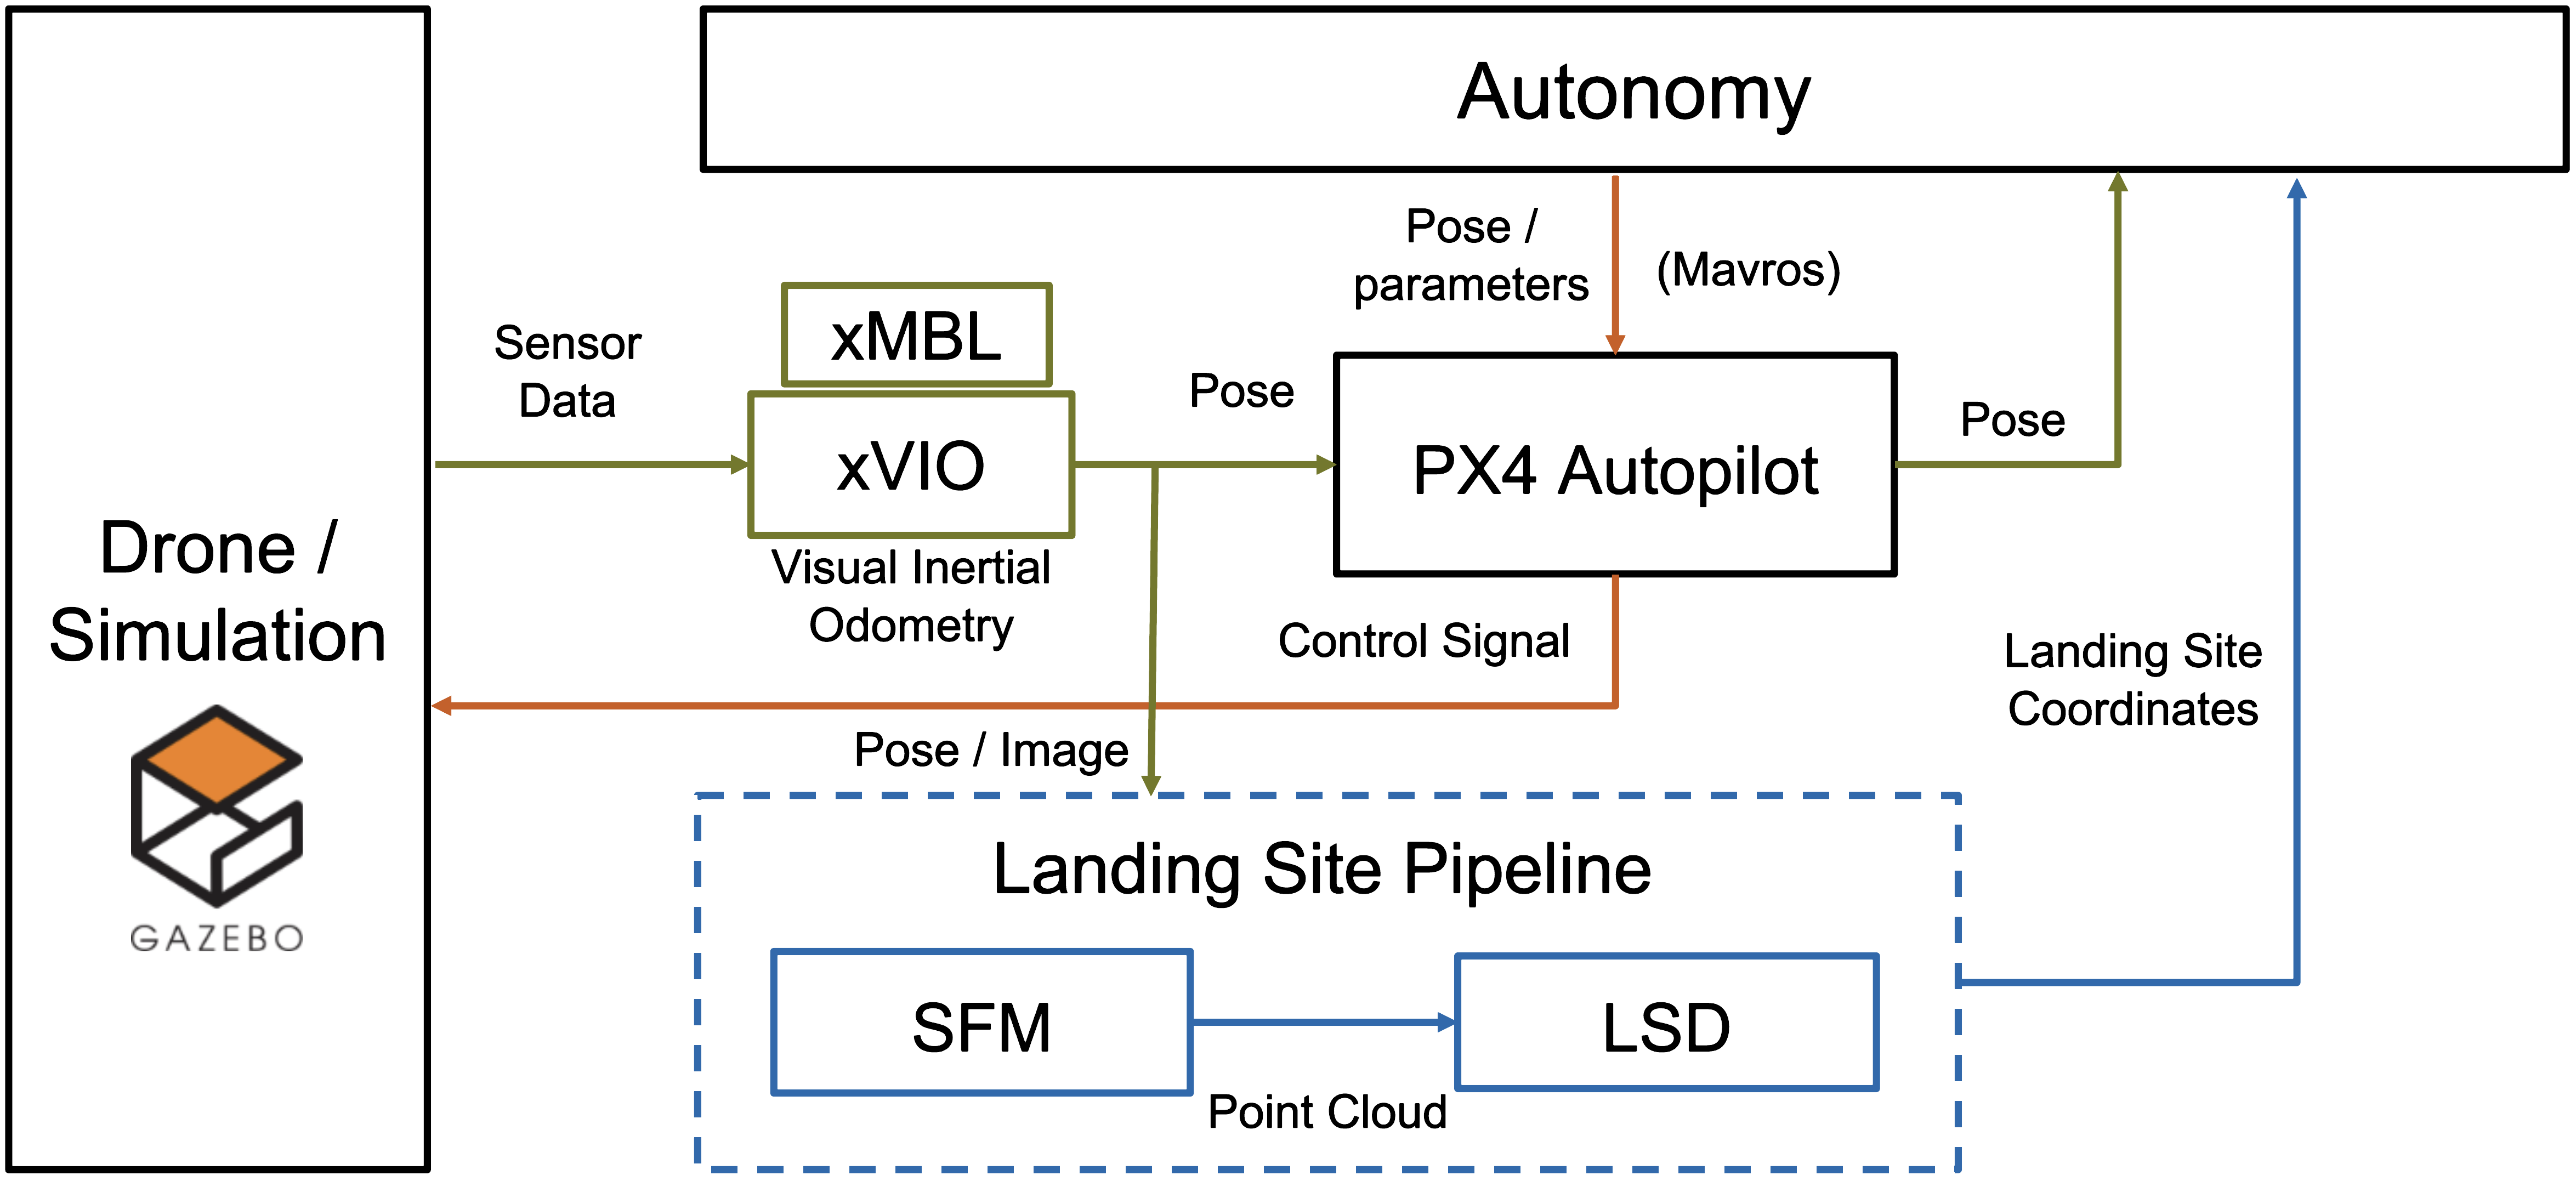
\includegraphics[scale=0.18]{images/system_overview/setup_flowchart_with_vio.png}
    \caption{LORNA Project Setup}
    \label{fig:lorna_setup}
\end{figure}

As the state estimator and the map based localization were not fully implemented at the time of this work, ground truth pose information from the simulated sensors was used instead. This is shown in \cref{fig:lorna_setup_GT_pose}

\begin{figure}[ht]
    \centering
    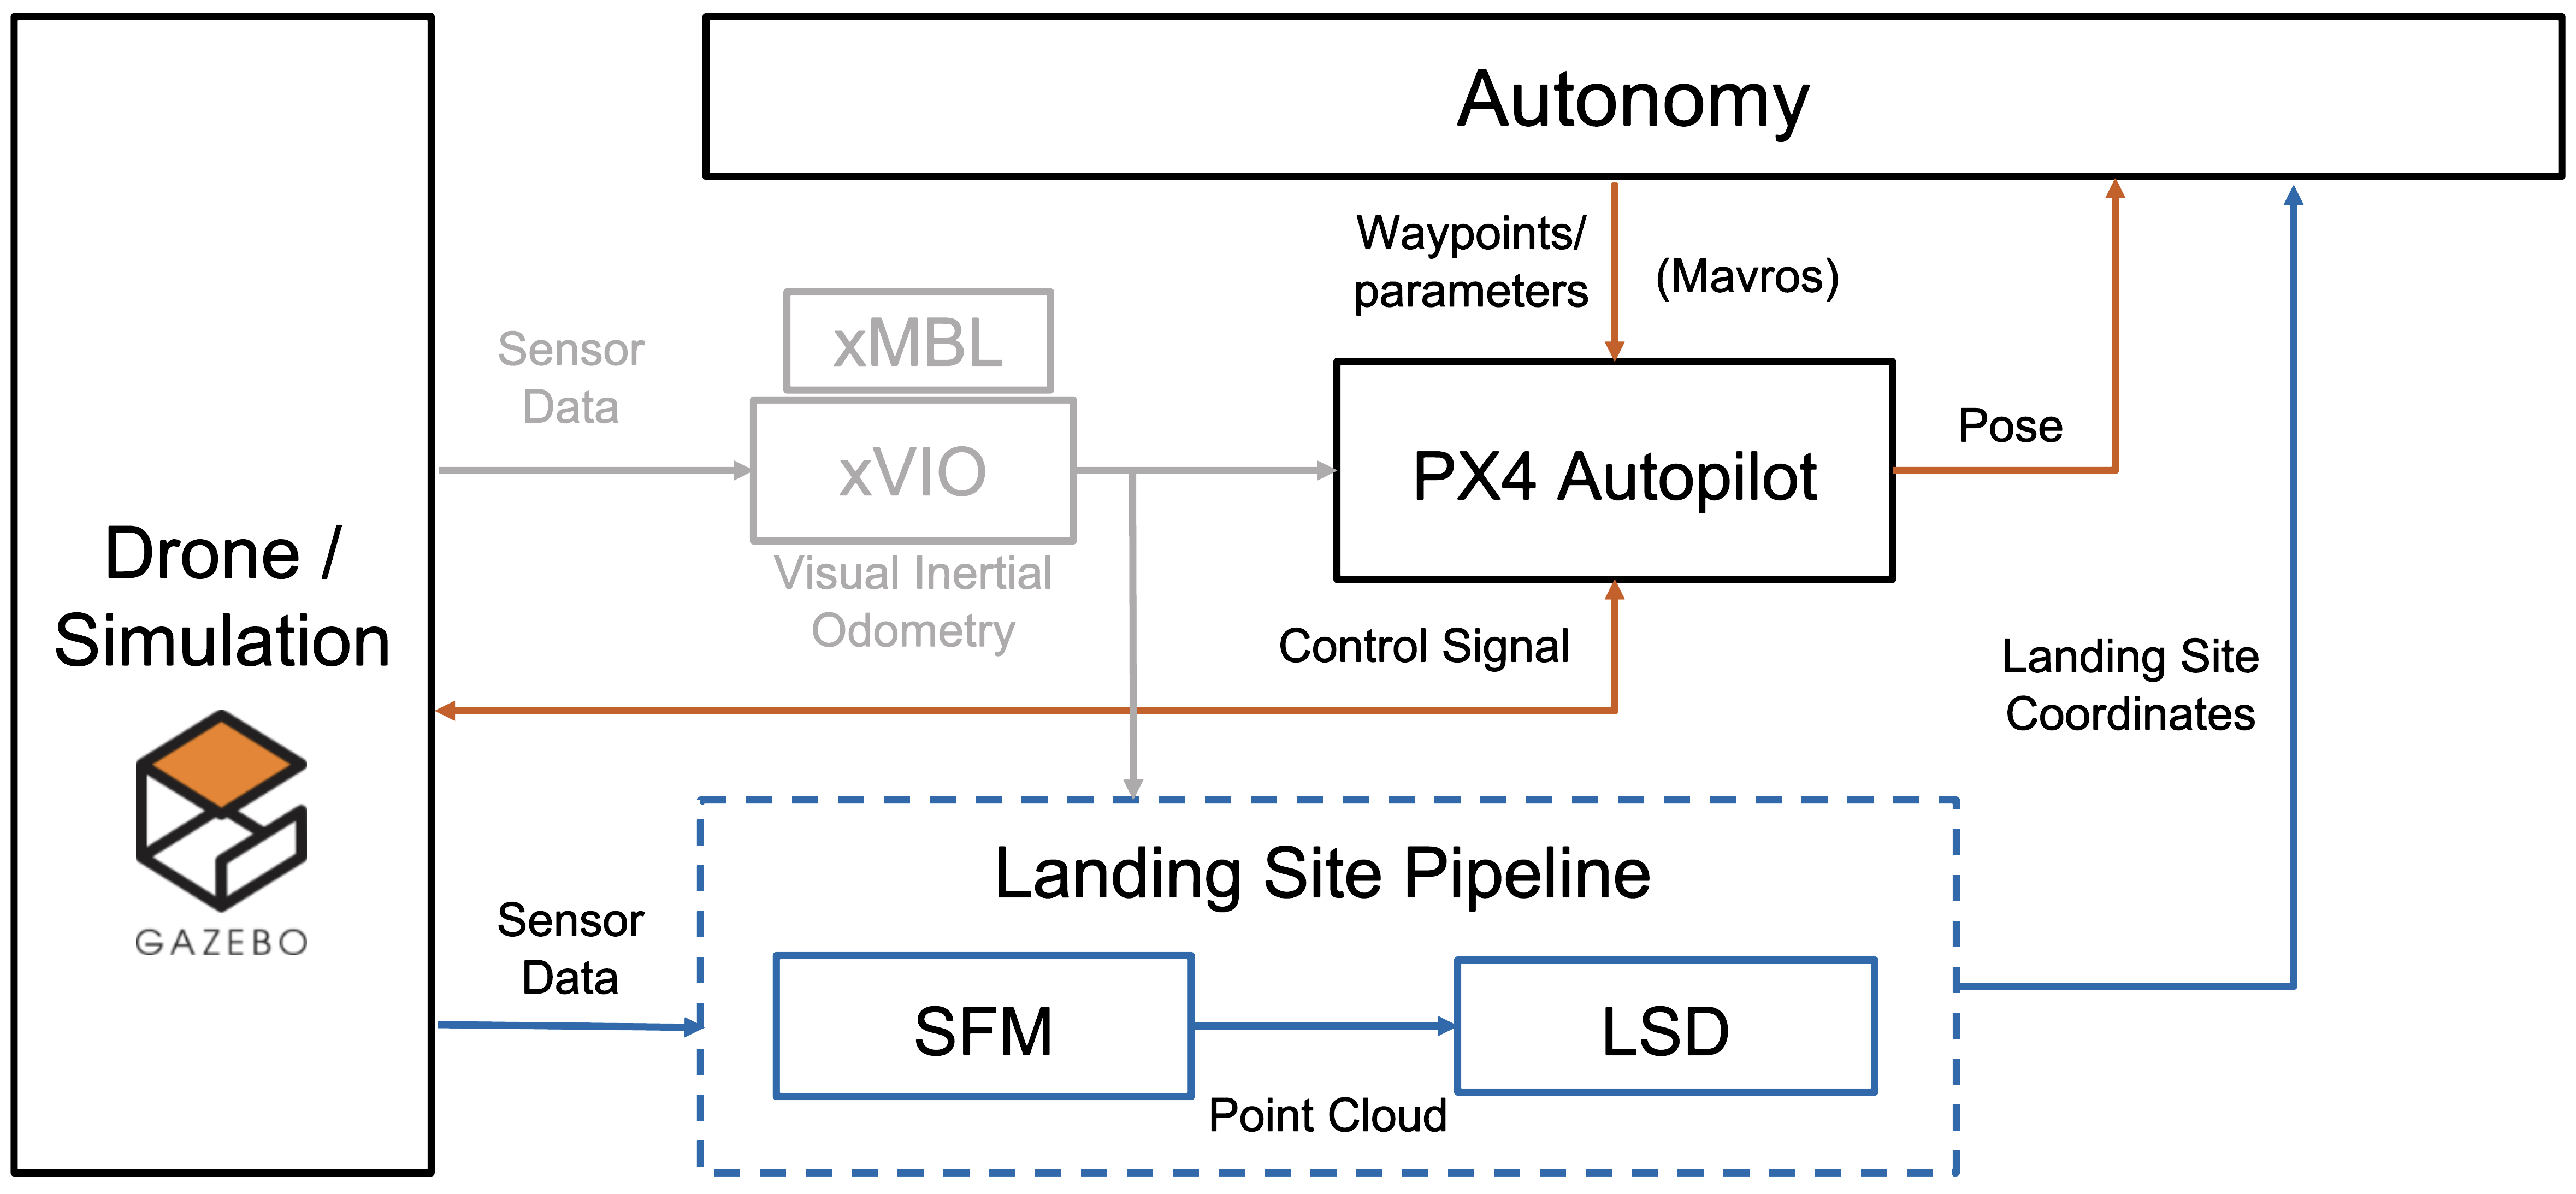
\includegraphics[scale=0.18]{images/system_overview/setup_flowchart.png}
    \caption{LORNA Project Setup with GT pose}
    \label{fig:lorna_setup_GT_pose}
\end{figure}

Since this thesis focuses on the integration of existing software instances, it is essential to delve into each component and elucidate their operational mechanisms.

\clearpage %HERE
\section{Simulation}\label{sec:simulation}

In this work I almost exclusively used a drone simulation. This allowed for a facilitated development with respect to both speed and safety. The choice of simulator, which is Gazebo Garden, was made prior to this work during the development of the autonomy.

\begin{figure}[ht!]
    \centering
    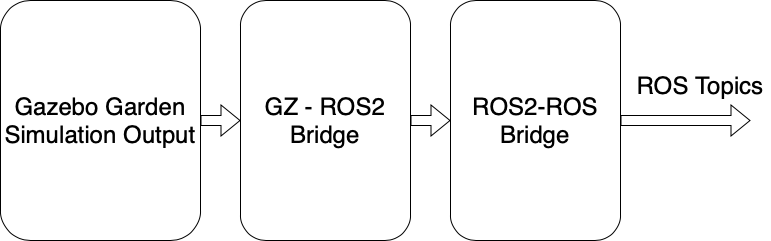
\includegraphics[scale=0.45]{images/system_overview/GZ_flowchart.png}
    \caption{Gazebo ROS Bridge}
\end{figure}


As the entire software stack of the LORNA project is dependent on ROS instead of ROS2, a bridge was used to convert the sensor information from Gazebo to ROS2 and from ROS2 to a ROS topic.

Most development during this work was performed on the Arroyo map shown in \cref{fig:arroyo_intro}. The Arroyo Seco is the area outside the Jet Propulsion Laboratory in Pasadena, California. Though, not a strikingly similar to Mars' landscape at first glance, the Arroyo contains varying terrain including small rocks and uneven ground which makes it a good test ground for UAV Mars landing applications.

\begin{figure}[ht!]
    \centering
    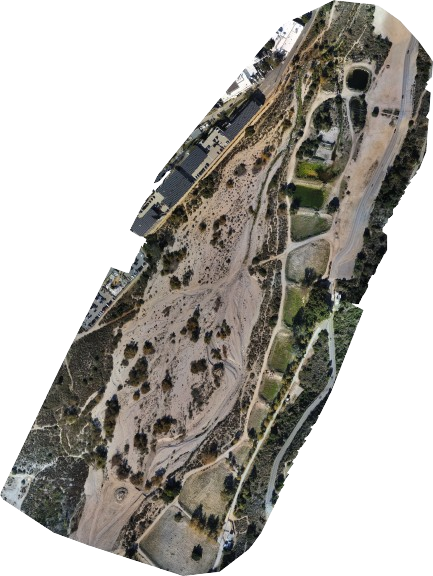
\includegraphics[scale=0.45]{images/evaluation/arroyo.png}
    \caption{Gazebo map of the Arroyo Seco area outside JPL at 4 cm per pixel}
    \label{fig:arroyo_intro}
\end{figure}


\section{Landing Site Detection Pipeline}\label{sec:setup:LSP}

The landing site detection pipeline consists of two nodes. A structure from motion node \citep{SFM} which creates a point cloud using a key frame based stereo depth approach on monocular images and a landing site detector algorithm \citep{LSD1, LSD2} which aggregates the depth measurements into a rolling buffer based multi-resolution elevation map and segments landing sites on the created DEM. These found landing sites are then supplied to the autonomy. 

\subsection{Structure From Motion (SFM)}\label{subsec:setup:SFM}

The structure from motion approach retains images and their associated pose priors as key frames in a sliding window buffer. These key frames are used for a bundle adjustment pose refinement and subsequently, using a previously stored key frame and the incoming pair, a stereo depth algorithm is applied to achieve a depth image. 

In the following, the three main parts are explained in more detail:

\subsubsection{Key Frame Handling}

At the end of an iteration the key frames are updated. Naturally, in the beginning before the rolling buffer is filled, each incoming frame is simply added to the back of the buffer queue. Upon reaching the queue's maximum capacity, incoming frames are analyzed regarding the two following factors:

\begin{itemize}
    \item \textbf{Frame to frame parallax}

    To ensure that enough distance has been covered between the last key frame and the incoming frame, the root-mean-square value for the parallax distance of the matched features is calculated and compared with a minimum threshold.
    \item \textbf{Information retention and contribution}

    To advance the buffer over time, new information should be added. Therefore, new features should be detected on an incoming image. To match the incoming image with the existing key frames however, sufficient features must also be shared with the previously detected key frames.
\end{itemize}

Therefore, if these two conditions are fulfilled, a new frame is accepted in the buffer. To determine the quality of the current key frames, the oldest key frame is used to determine the following metrics:

\begin{itemize}
    \item \textbf{Number of matched features between the two frames}
    \item \textbf{Overlap of the two image footprints}
    
    Using the simple pinhole model formula for an image footprint and the calculated baseline, the overlap of the areas are calculated.
    \item \textbf{Feature area ratio}
    
    The maximum rectangle spanning all features is derived for both frames. Due to parallax from lateral motion, they don't overlap allowing to determine the area ratio of the feature span overlap.
\end{itemize}

If these three metrics lie above a certain threshold, the key frames are considered good and only the newest key frame is exchanged, retaining all others. If not, the new frame is added to the back, pushing the rolling buffer further, leading to the loss of the oldest previous key frame. 

\subsubsection{Bundle Adjustment}

Before doing 3D reconstruction, the poses are refined using a bundle adjustment algorithm. This is beneficial as the state estimator will always come with a certain error which drifts over time. 

\begin{figure}[ht!]
    \centering
    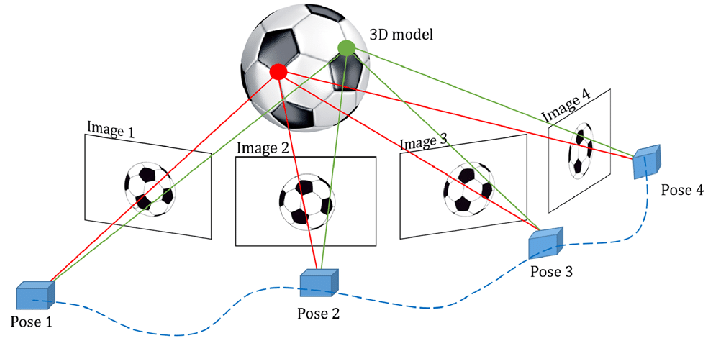
\includegraphics[scale=0.5]{images/system_overview/BA.png}
    \caption{Bundle Adjustment Procedure as shown in \citet{BA}}
    \label{fig:BA}
\end{figure}

\cref{fig:BA} shows the change in reprojection, which the bundle adjustment optimization technique thrives to diminish. Generally, it does so by considering a number of key frames and optimizing their poses as well as the camera parameters used to acquire the images. In this case, only the pose refinement is considered for the key frames in question.

\subsubsection{Stereo Depth}\label{subsubsec:SFM_stereo}

Having chosen adequate key frames and refined their poses, the crucial step of 3D reconstruction can be performed. For this, the key frames are checked to have an image overlap with the new image that is sufficient but not fully overlapping and to have a small enough baseline inclination so that assuming the same altitude above ground is reasonable. If the checks are successful, the key frame with the largest baseline to the new frame is chosen for the stereo procedure. 

Note that if all key frames comply with these checks than always the oldest key frame is used for the stereo depth creation. Therefore, in practice the reference view for the depth image is the oldest key frame for a few iterations until the overlap with the new image is too small, and the oldest key frame is switched out. This results in a small jump of the depth image's reference location. 

\begin{figure}[h]
\centering
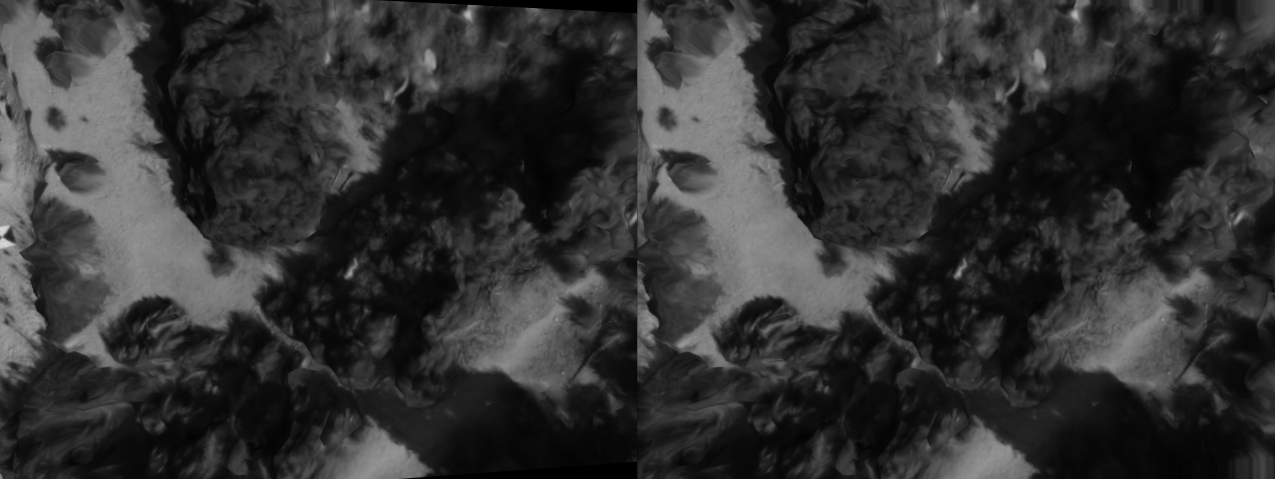
\includegraphics[scale=0.28]{images/system_overview/sfm_images.png}
\caption{Left and right key frame image selected for SFM depth}
\label{fig:sfm_images}
\end{figure}

\cref{fig:sfm_images} shows a selection of such key frames to perform stereo on. Not the visible rectification in the left reference image which has been rotated slightly in order to enable horizontal feature matching.

Using the two frames and the parallax distance between the detected features due to lateral motion between the images, the disparity values can be derived. With the camera's intrinsic parameters and the disparity values, a depth image of the terrain can be created. A color coded example thereof is shown in \cref{fig:sfm_depth_image} where red points are closer and blue ones further away from the camera sensor.

\begin{figure}[h]
\centering
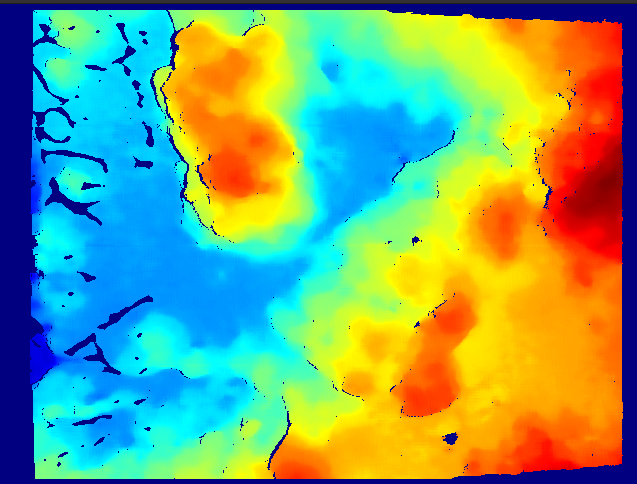
\includegraphics[scale=0.45]{images/system_overview/sfm_depth_image.png}
\caption{SFM depth image created from the stereo approach}
\label{fig:sfm_depth_image}
\end{figure}

Then, using these depth values of the individual and the camera parameters, the 3D coordinates of each detected point can be calculated, and thus the depth image is converted into a point cloud which is the format required for LSD. The RViz visualization of such a point cloud is shown in \cref{fig:sfm_point_cloud}.


\begin{figure}[h]
\centering
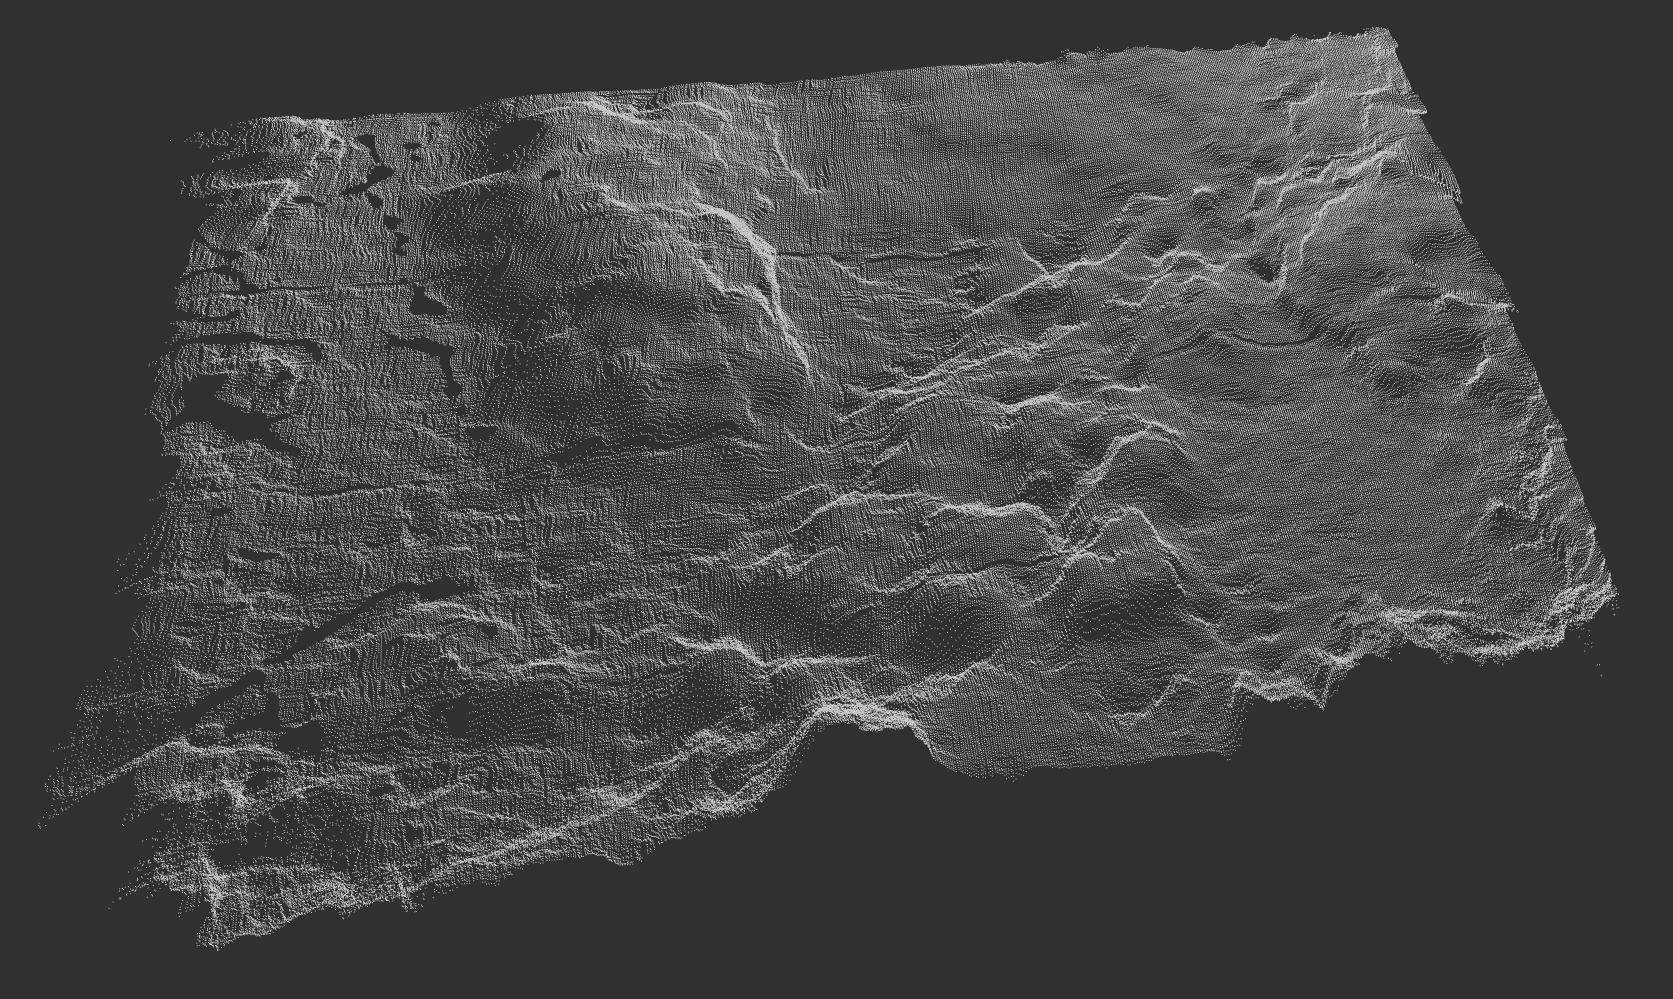
\includegraphics[scale=0.2]{images/system_overview/sfm_depth_map.png}
\caption{SFM point cloud visualization in RViz}
\label{fig:sfm_point_cloud}
\end{figure}

\subsection{Landing Site Detection (LSD)}\label{subsec:setup:LSD}

\subsubsection{Depth Aggregation}\label{subsubsec:setup:aggregation}

The foundation of the landing site detection mechanism is a rolling buffer based multi-resolution elevation map as indicated in \cref{fig:DEM}. Each base layer cell is represented with 4 cells at a higher resolution layer.

\begin{figure}[ht!]
    \centering
    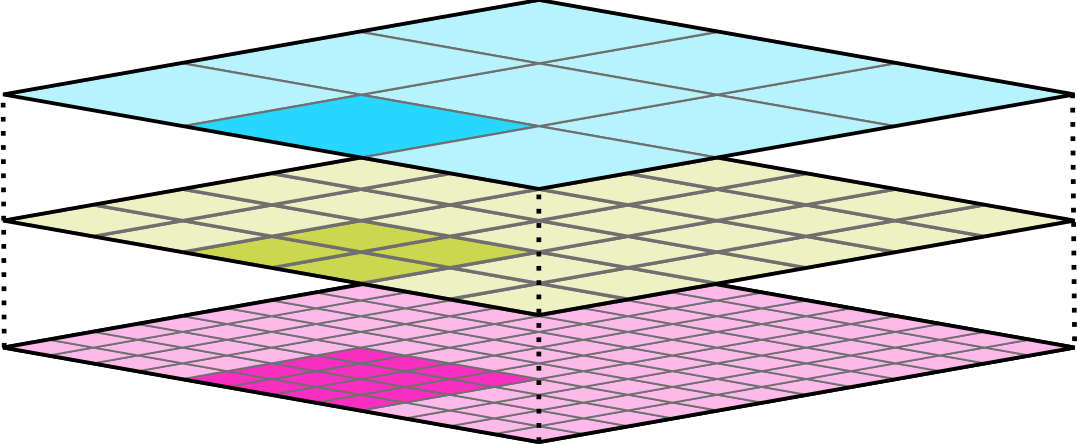
\includegraphics[scale=0.25]{images/system_overview/DEM.png}
    \caption{Multi resolution elevation map as displayed in \citep{LSD1}}
    \label{fig:DEM}
\end{figure}

As introduced in \citet{LSD2}, each cell in this dense elevation map (DEM) is composed of an optimal mixture of Gaussian (OMG) state described by the following three variables:

\begin{itemize}
    \item $\mu$ - The mean of the depth at this cell
    \item $\sigma^2$ - The variance of the depth measurements
    \item $S$ - An auxiliary variable to keep track of past measurement's uncertainties
\end{itemize}

Each point cloud input iteration, a depth measurement and the associated stereo depth uncertainty is received. The measurements are placed in the respective cells based on the level of detail (LoD) of the perceived points. The LoD being $\frac{z}{f}$, where z is the depth measurement and f is the focal length of the camera. Specifically, an incoming measurement is placed in the highest resolution layer of all layers which are coarser than the incoming measurement. If the measurement has a larger pixel footprint than any of the layers, it is entered in the coarsest layer which is the top.

In a subsequent step the measurements are pooled up to the top layer and down again in order to make the DEM more consistent and interpolate missing values. The same result could be achieved by entering each measurement individually and directly pooling it up and down the cells that cover its footprint. However, splitting the procedure into a step that acquires all measurements and second task that collectively pools all cells, achieves the same with fewer updates.

Similar to Kalman filters, the OMG cells' uncertainties improve over time as more measurements are entered. Because of this the DEM's terrain estimate converges over time. This is beneficial for the acquisition of landing sites on well known terrain. However, convergence on known terrain makes it harder for future inputs to override the existing DEM. To counteract this \citet{LSD2} proposed a time inflation factor which was however not implemented. This would reduce the weight of older data and make it thus easier for incoming points to alter the cells.

When an incoming point cloud comes from a camera pose which yields less than 95\% theoretical image overlap with the previous location, a map shift of the rolling buffer is performed. The rows and columns no longer necessary are cleared, and the starting index is shifted for further incoming point clouds. This implementation allows the movement of the map without the need to reassign filled cells. In other words, by merely reassigning the cell values of the DEM container, the required parallax effect is achieved.

This shift is visualized in \cref{fig:map_movement}. Note the images\footnote[1]{Images were created using DeepAI's image generator (https://deepai.org/machine-learning-model/text2img)} are only used for ease of demonstration. They represent incoming point clouds. The dashed orange arrow indicates the drone's movement relative to the instantaneous DEM. The new Image is entered at the new starting index and points exceeding the map boundaries are wrapped around to the other side. The part of the DEM which was deleted is filled with the incoming points and new measurements at the location of retained information lead to an update of the previously filled cells. Note that \cref{fig:map_movement} shows a very radical map movement. Smaller camera movements between iterations would lead to the retention of most of the DEM.

\begin{figure}[ht!]
    \centering
    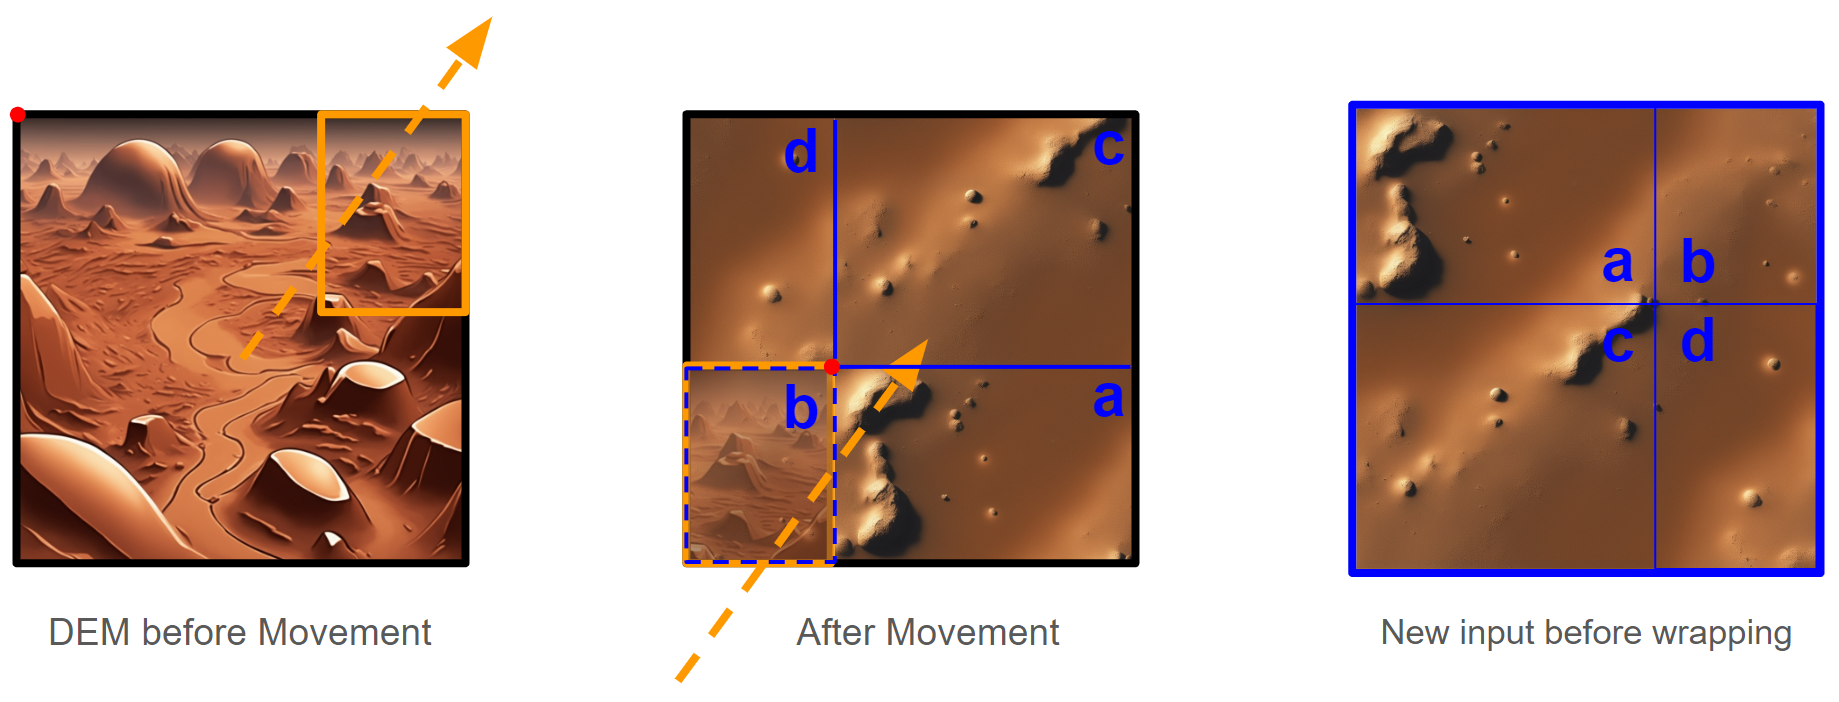
\includegraphics[scale=0.25]{images/system_overview/map_movement.png}
    \caption{Schematic LSD map movement procedure: Outlined with orange is the retained part of the DEM (in the second frame it is overlaid by part of the new input). The blue image represents the next input point cloud and the red dot indicates the starting index where the new point cloud starts to be stored. Both images were created using AI.}
    \label{fig:map_movement}
\end{figure}


\subsubsection{Hazard Segmentation}\label{subsubsec:setup:haz_seg}

On this created DEM, landing sites are then detected. This is done using a roughness and slope assessment of the perceived terrain. Roughness defines the maximum absolute altitude difference around a cell for a given resolution layer and slope is determined by fitting a plane to the vicinity of a considered point.

The roughness check is done for each resolution layer of the DEM. To assess the roughness around a cell, all surrounding cells within a predefined proximity threshold are considered, and the maximum value is stored. The computational cost of the hazard segmentation is dominated by the roughness checks at the lower layers. Therefore, to make it more efficient, a minimum and maximum buffer were introduced respectively. This allows to store the extreme values at a given location and then for the roughness assessment of a neighboring cell, the knowledge about that mostly overlapping area can be used. With this, only the new margin of cells has to be considered for minimum/maximum candidates of subsequent cells. Finally, the roughness of a cell is the difference between the maximum and minimum value in that cell's vicinity.

A visualization of this procedure is shown in \cref{fig:lsd_roughness_check}:

\begin{figure}[ht!]
    \centering
    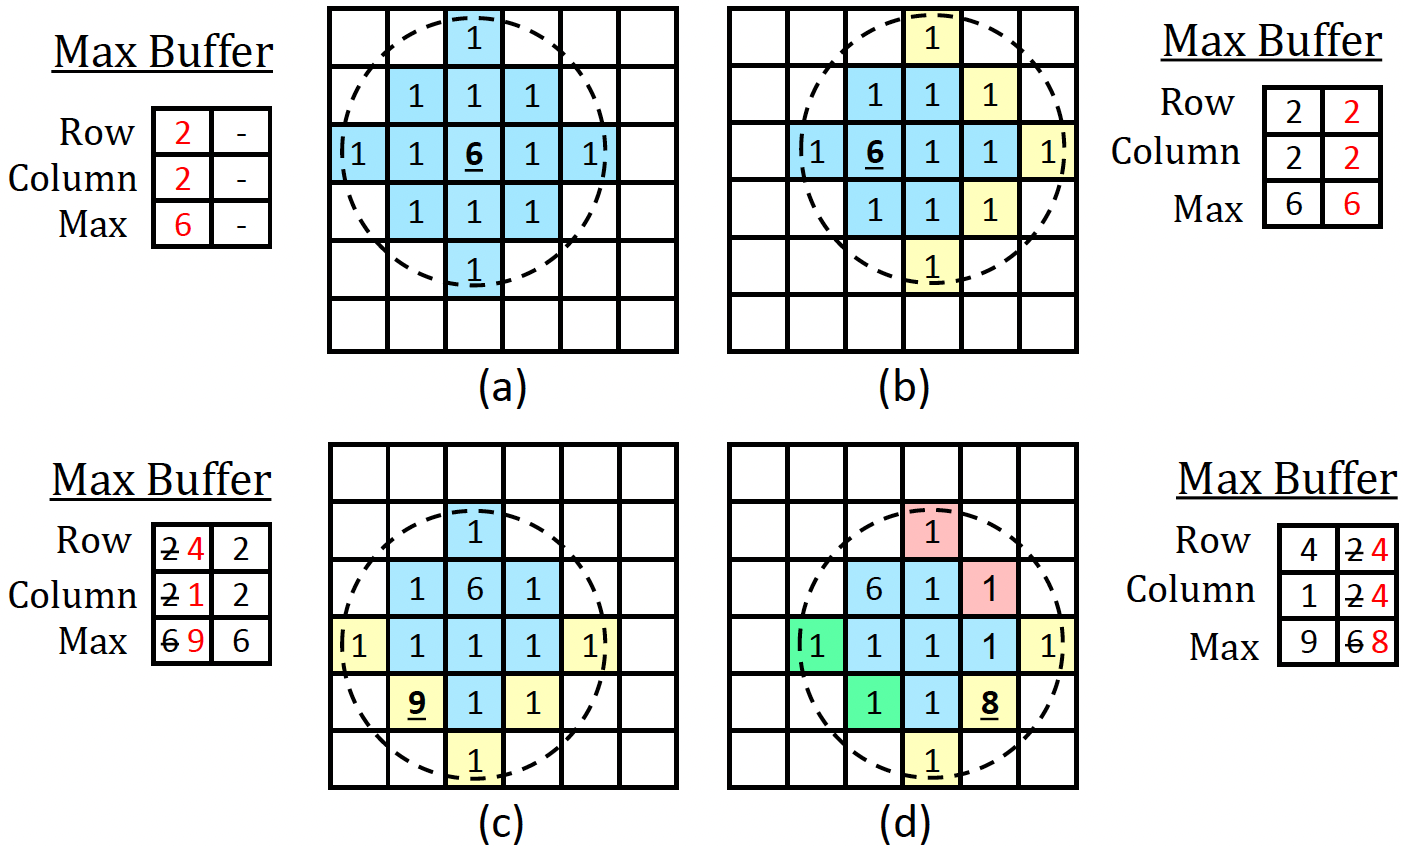
\includegraphics[scale=0.5]{images/system_overview/roughness_check.png}
    \caption{Optimized roughness assessment as shown in \citet{LSD2}}
    \label{fig:lsd_roughness_check}
\end{figure}

As the slope of a location depends on a larger encompassing area around a cell, the assessment of the slope at the highest (coarsest) layer is sufficient. For each cell in the top layer and the area surrounding it, a plane is fitted using the linear least squares equation $Ax = b$ where A is a matrix containing in each row the x and y coordinates as well as a homogeneous coordinate for the plane's offset. The solution vector x contains the plane's properties $\left(N_x, N_y, d\right)$ where $N_x$ and $N_y$ define the plane's normal vector's orientation and $d$ is the plane's offset. Note that $N_z$ was fixed to be 1. The maximum inclination can then be calculated as the angle between the normalized normal vector and the z axis $\theta = \arccos\left(\frac{N \cdot e_z}{||N||}\right)$

If the roughness and inclination values lie within the acceptance threshold, the spot is recognized as a landing site and marked as such in a binary landing map. 

\begin{figure}[ht!]
    \centering
    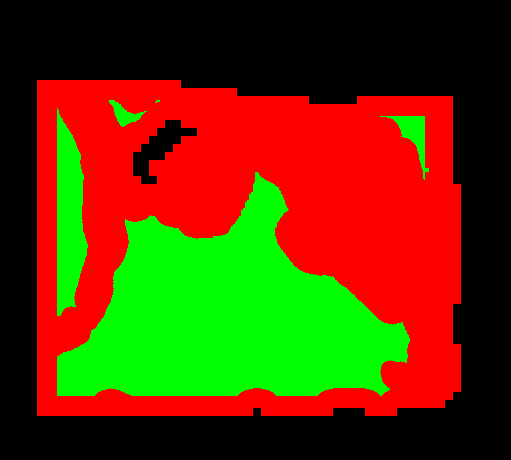
\includegraphics[scale=0.5]{images/system_overview/landing_map.png}
    \caption{Binary landing site map from the LSD debug image. Black is terrain not yet covered, red are invalid landing sites and green are detected valid landing sites.}
    \label{fig:ls_map}
\end{figure}

\subsubsection{Landing Site Selection}\label{subsubsec:setup:ls_select}

After applying a distance transform on the landing site map, which yields the minimum pixel distance to a non-landing site, non-maximum suppression is performed. In this maximum peak detection only N landing sites are selected which have a size that is at least bigger than the largest landing site multiplied by a certain diminutive factor and are sufficiently far away from another peak to be considered an actually distinct landing site.

\begin{figure}[ht!]
    \centering
    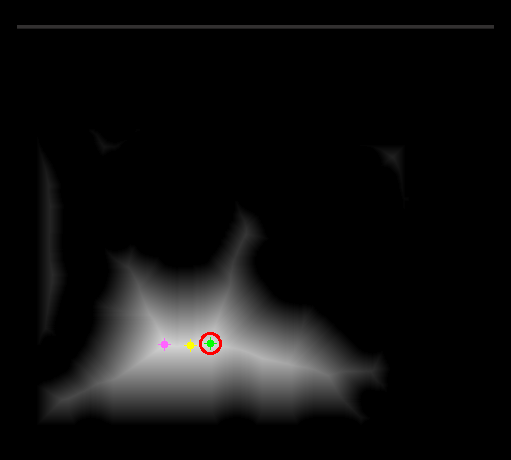
\includegraphics[scale=0.5]{images/system_overview/non_max_suppression.png}
    \caption{Non-maximum suppression: the three best landing sites at any given iteration are chosen of which the very best is encircled.}
    \label{fig:non_max_sup}
\end{figure}

Lastly, their positions are refined by applying a mean shift algorithm for a few iterations. This algorithm uses a Gaussian kernel which considers the roughness, normalized distance transform and the uncertainty of the cells in the sampled region. The exact implementation is shown in \citet{LSD2}. The selection of multiple peaks at any given time is useful, as the mean shift algorithm is prone to local minima. So having multiple candidates and applying the mean shift algorithm to each one individually, makes the selection of a good landing site more probable.

\begin{figure}[ht!]
    \centering
    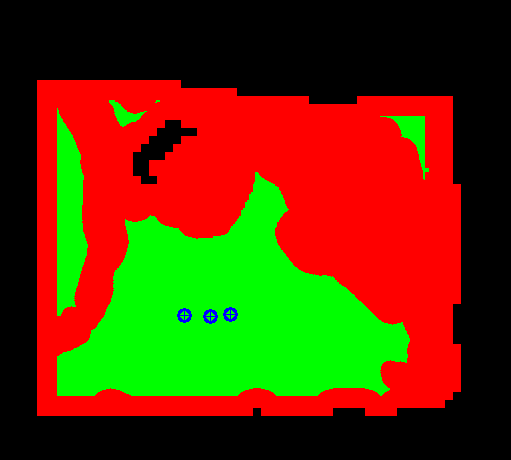
\includegraphics[scale=0.5]{images/system_overview/landing_map_marked.png}
    \caption{Binary landing site map after non-maximum suppression}
    \label{fig:ls_map_nps}
\end{figure}

\cref{fig:ls_map_nps} shows the landing map with the final shifted maximum area landing sites. These optimized landing site candidates are indicated with the blue crosses. 

\clearpage %HERE

\subsubsection{Debug Images}

\begin{figure}[ht!]
    \centering
    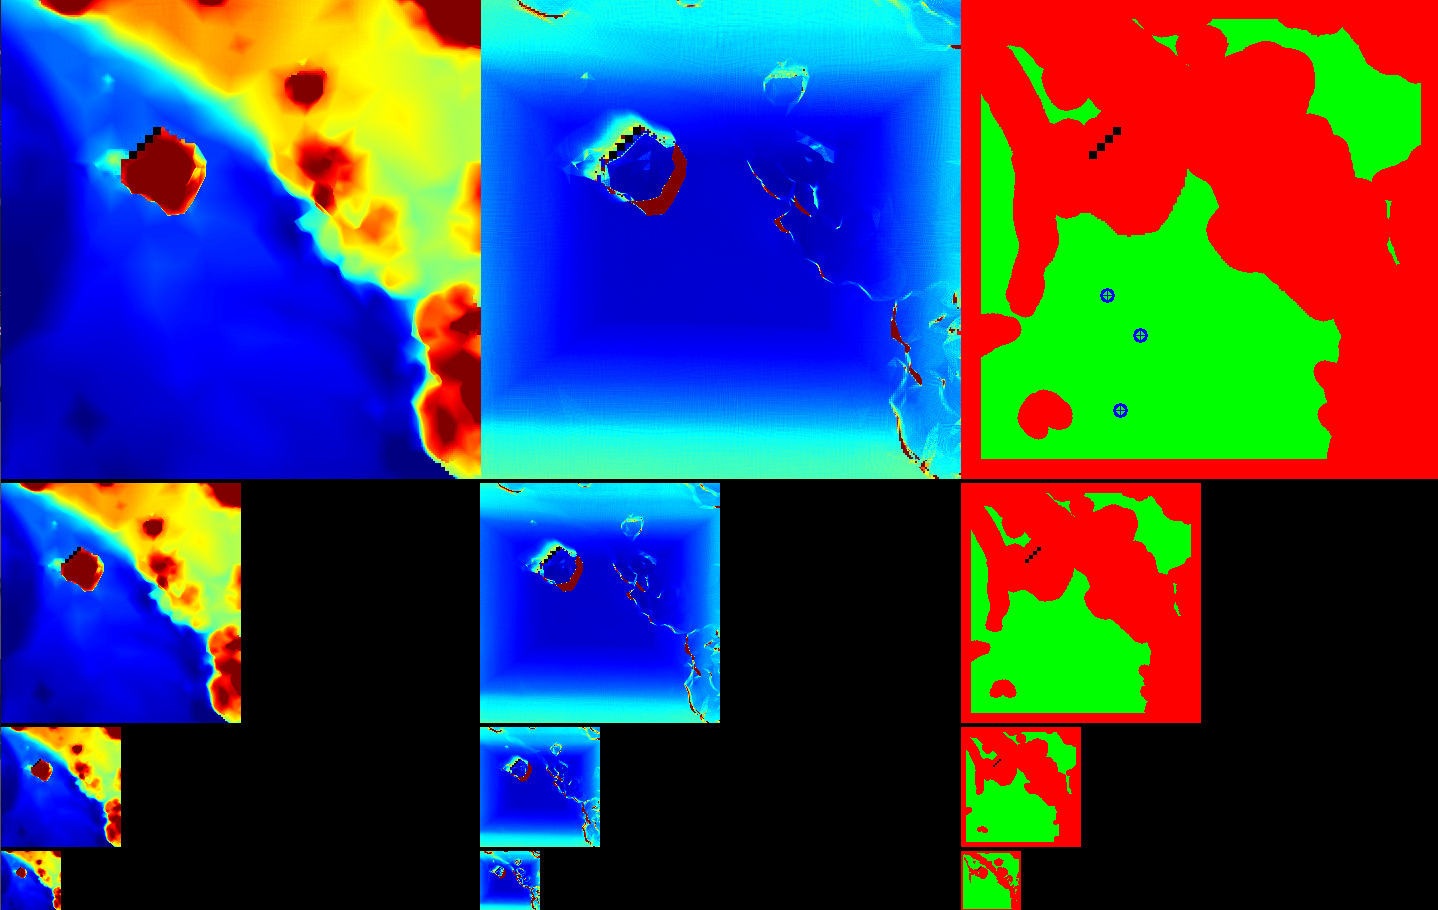
\includegraphics[scale=0.25]{images/system_overview/lsd_debug_image.png}
    \caption{LSD Debug Image - Left: DEM, Middle: Uncertainties, Right: LS Map}
    \label{fig:lsd_debug} %Replace with SFM LSD image here
\end{figure}

\begin{figure}[ht!]
    \centering
    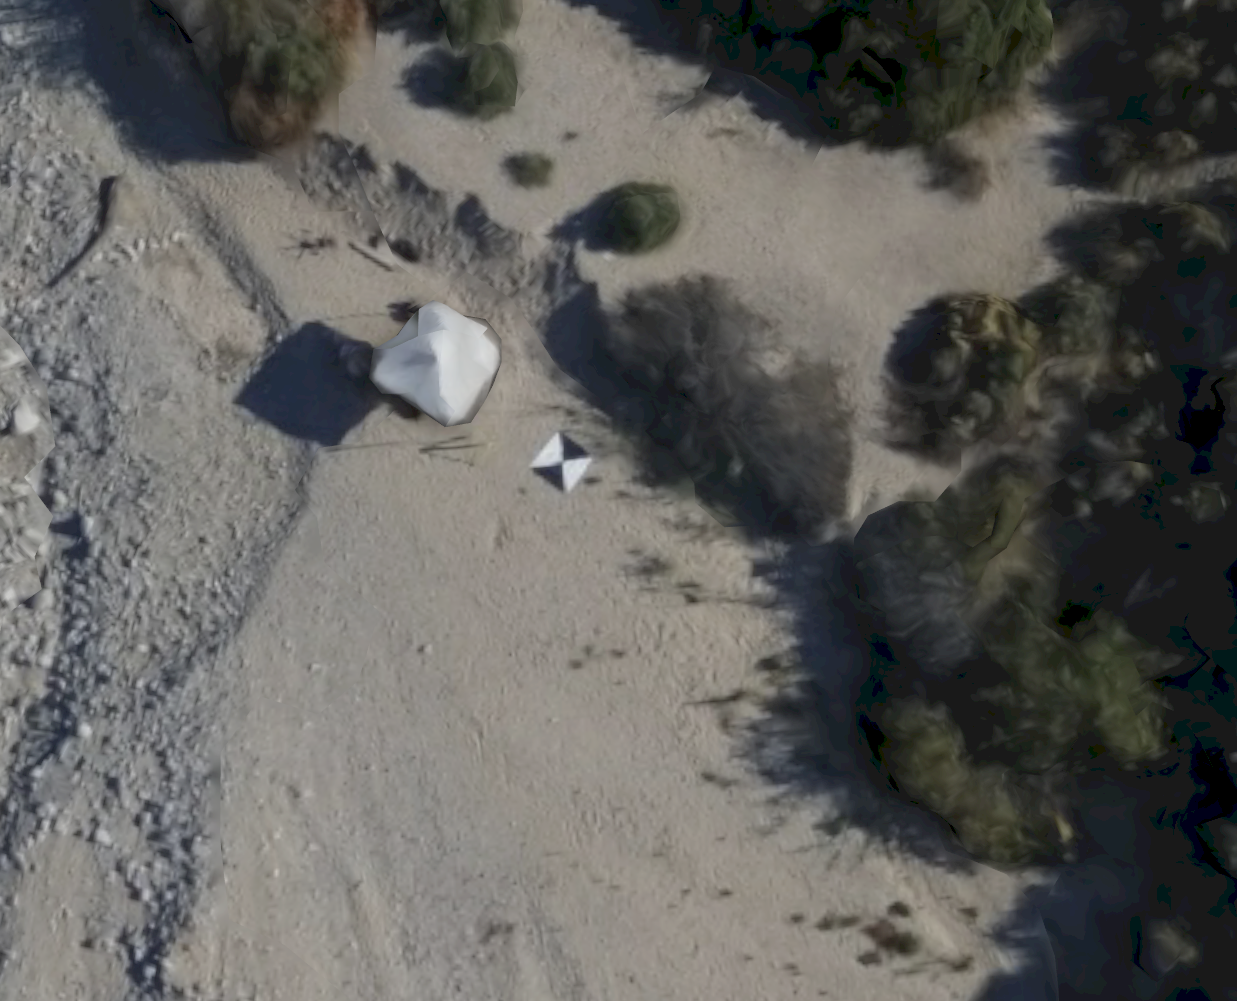
\includegraphics[scale=0.25]{images/system_overview/lsd_debug_reference.png}
    \caption{Gazebo Simulation Reference}
    \label{fig:lsd_debug_ref}
\end{figure}

The landing site detection debug image is a good comprehensive visualization of the landing site detection algorithm. 

On the left, one can see the multi-resolution map displaying the same terrain area in different resolutions. Red pixels are closer, blue further away.

In the middle one can see the uncertainties of the detected points. Blue signals a low uncertainty while red denotes a high uncertainty. 

On the right is the above-mentioned binary landing site map. Green indicates valid landing sites, and the blue crosses indicate the chosen non-maximum suppressed and mean shifted landing sites.   

\section{Autonomy}\label{sec:setup:autonomy}

The autonomy framework was developed within the LORNA project as a master's thesis by my friend and colleague Luca Di Pierno (\citep{Autonomy}). It is the overarching instance governing all the necessary behaviors during a mission and constituting the interface between all the nodes of the navigation pipeline.

A visualization of the setup is shown in \cref{fig:autonomy}.

\begin{figure}[ht!]
    \centering
    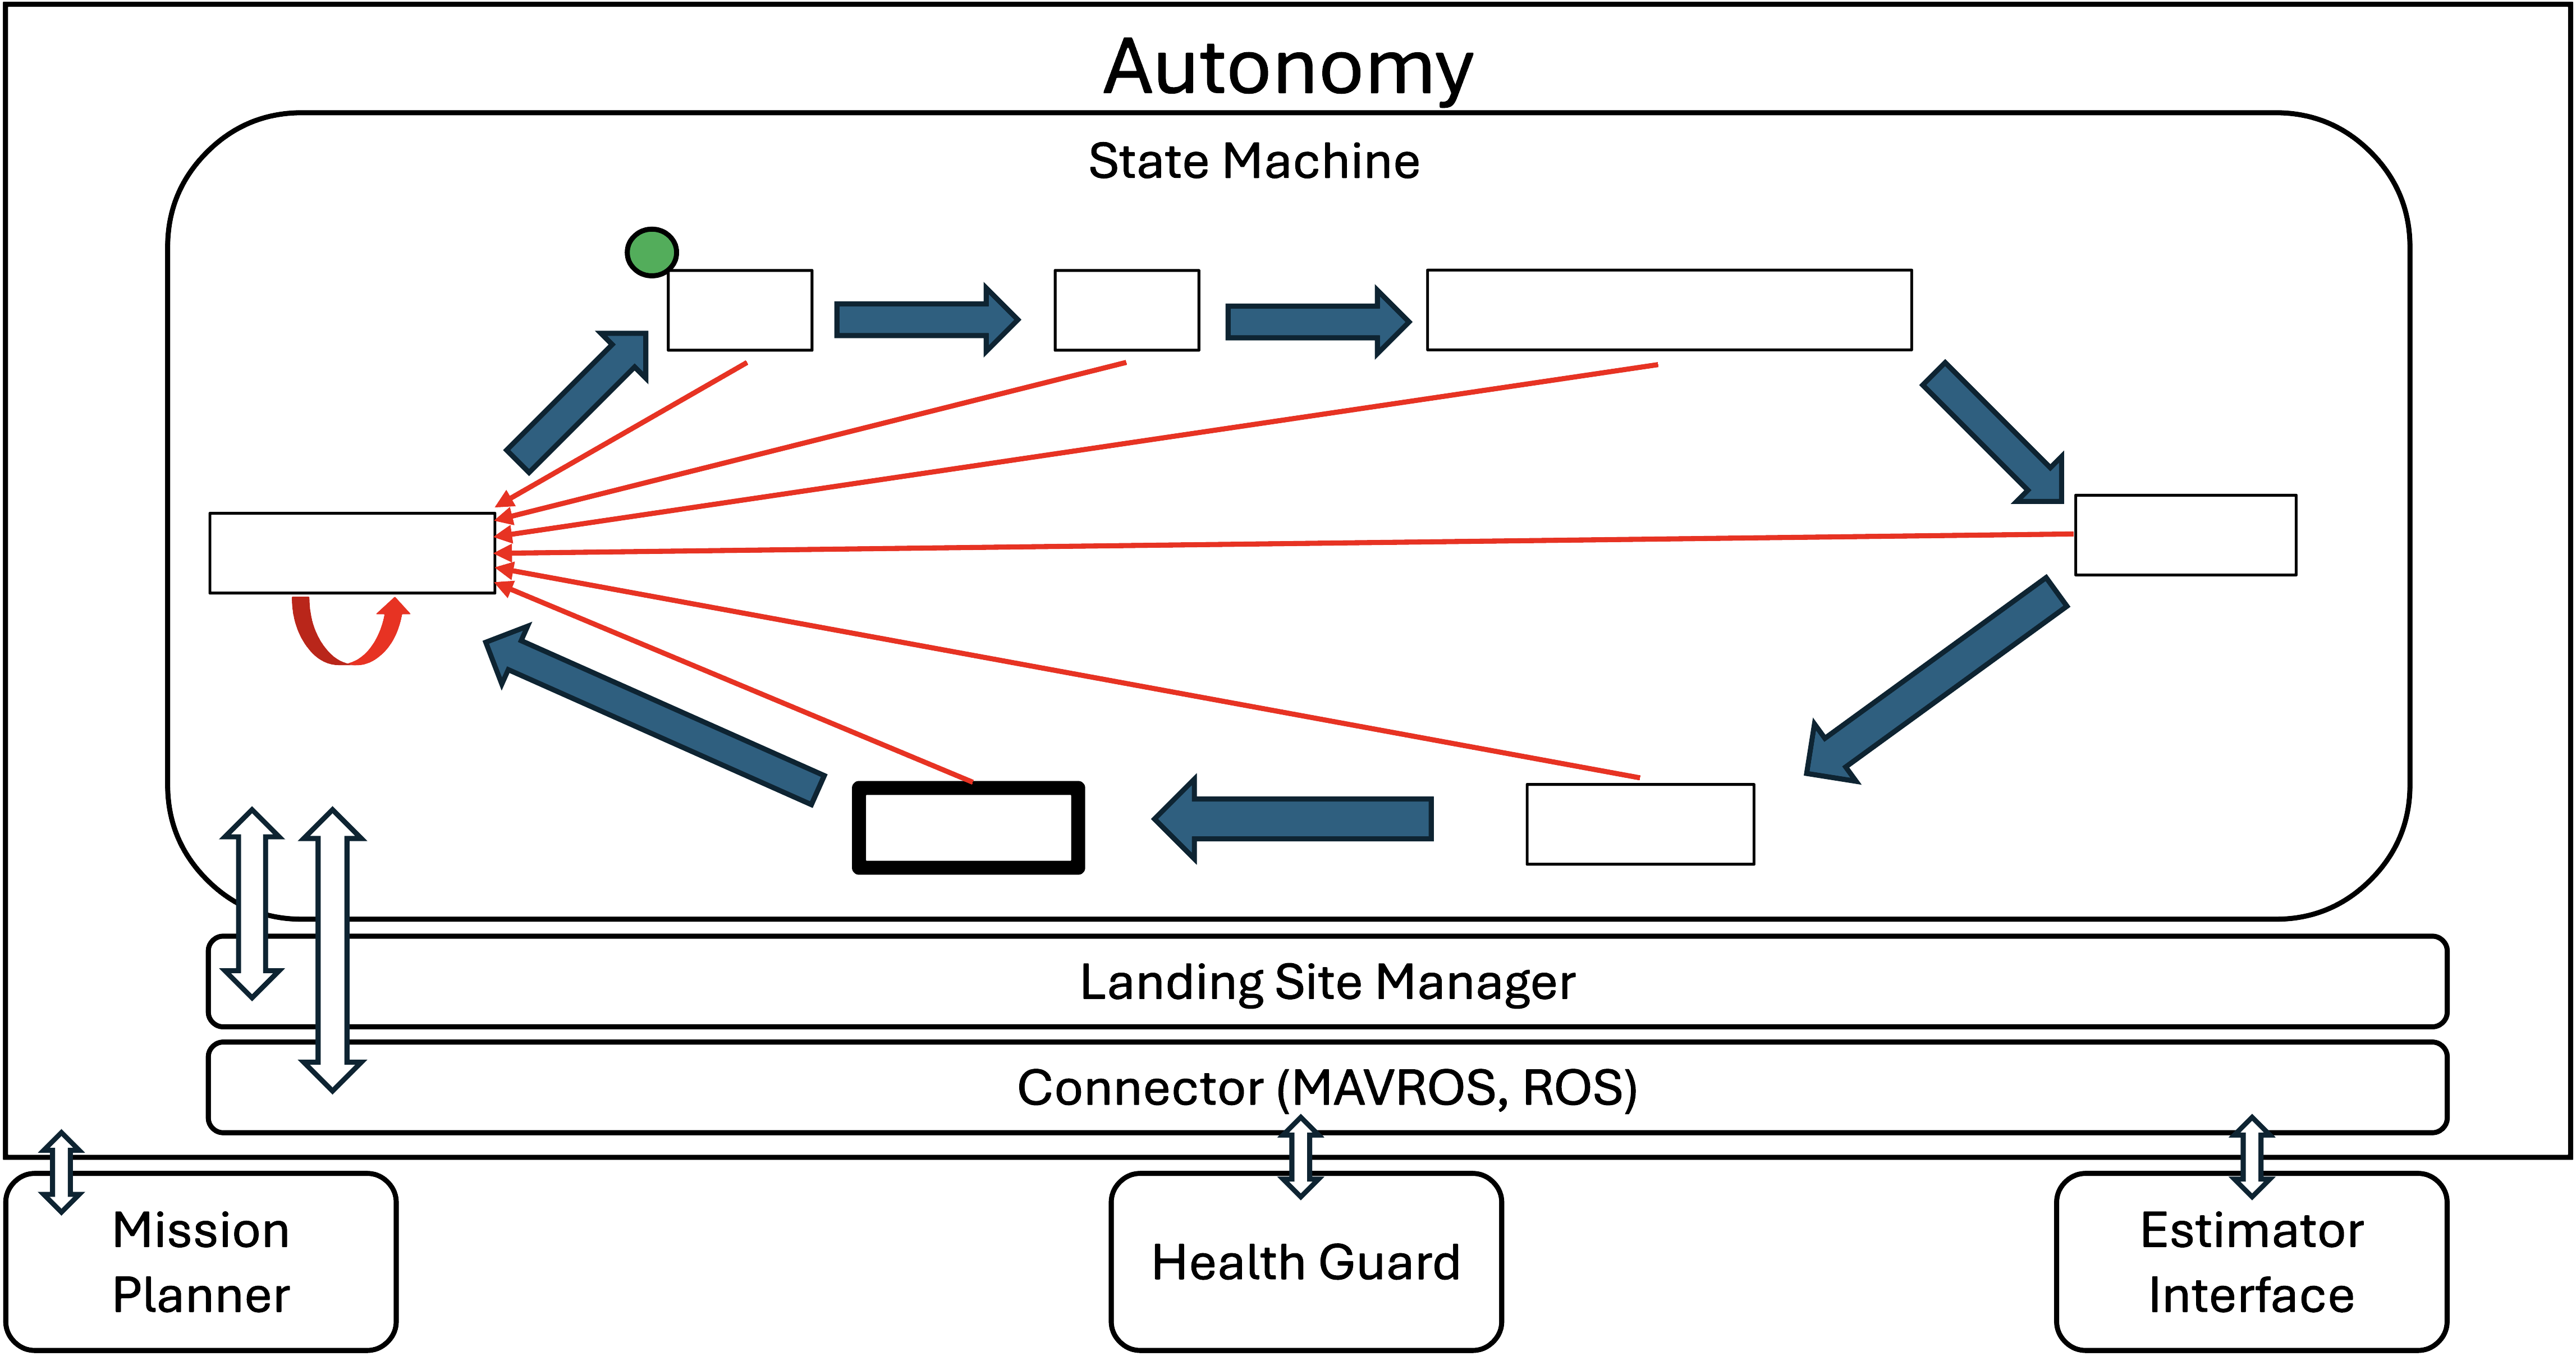
\includegraphics[scale=0.155]{images/system_overview/autonomy.png}
    \caption{Simplified overview of the autonomy}
    \label{fig:autonomy}
\end{figure}

As shown in \cref{fig:autonomy}, the core of the autonomy framework is a finite-state machine that reactively orchestrates task execution, ensuring that the individual actions are carried out in an organized and structured manner. Alongside the state machine there are two separate entities. A connector and the landing site manager. Lastly, a blackboard module is used to transfer information between states of the state machine.

\subsection{Support Nodes}\label{subsec:sup_nodes}

The autonomy framework is aided by three support nodes. These are shown at the bottom of \cref{fig:autonomy}:

\begin{itemize}
    \item Mission planner

    As the name suggests, the mission planner enables the easy packaging of a mission's waypoints into a format that the autonomy can parse and understand. For this, it needs merely a plan file from a ground station such as the used QGroundControl in this work. From this, the mission CSV file is created with the plain navigation information required to fly the desired course. Furthermore, the mission planner allows the user to add additional tasks to a mission waypoint. This allows for the very fast creation of missions with the potential modular enhancement of waypoints for science tasks.
    \item Health Guard
    
    This node is a notification tool which alerts the autonomy in case of a health issue of the system. This could be a range of events such as an actuator failure or simply a low battery level. The connection to the autonomy is established using a ROS service in the ROS connector interface (\ref{subsubsec:connector}). Each autonomy tick, the health state is queried using the ROS service. In case of an issue, the autonomy assesses the gravity of the issue and, in case of an emergency, initiates the reactive behavior.

    \item Estimator Interface
    
    This is the auxiliary node which handles the localization inputs. It is designed to be able to handle incoming pose estimates from different sources such as GPS, Vicon (a motion capture based localization system) and LORNA's xVIO estimator. In this work, apart from occasional autonomy tests on the hardware using the Vicon system and a field test using GPS, the estimator interface was not used, and the flights were performed on the flight controller's pose which is the simulations ground truth pose.
\end{itemize}

\subsection{Autonomy Interface}
\subsubsection{Connector}\label{subsubsec:connector}

The connector consists of two parts and constitutes the interface with the other software instances of the project:

The MAVROS connector establishes the off board mode in the PX4 autopilot in order to control the parameters and waypoints through the autonomy directly, effectively replacing the flight controller's decision-making behavior. It performs the arming and disarming procedure and executes actuator checks among other tasks to enable a rotorcraft flight.

The ROS connector receives health events about the system's status from the health guard node, the drone's current pose from the flight controller's state estimator and, crucial for this work, the detected landing sites from the LSD algorithm.

\subsubsection{Landing Site Manager}\label{subsubsec:LSM}

In parallel to both the state machine and the connector, the autonomy contains another separate entity, the landing site manager. 

It consistently processes the incoming landing sites from the LSD algorithm which were received by the ROS connector. During this processing, each landing site's distance to the drone's current position is calculated, and each landing site is assigned a heuristic value and ordered according to that value in the landing site buffer. This buffer is implemented as a min-heap. This allows the replacement and ordering of a new landing site with comparatively small overhead. 

Prior to this work, the heuristic used for comparison was simply the distance to the drone's current position resulting in the consistent choice of the closest landing site. 

The landing site manager's site processing is depicted in \cref{fig:lsm_ls_processing}

\begin{figure}[h]
\centering
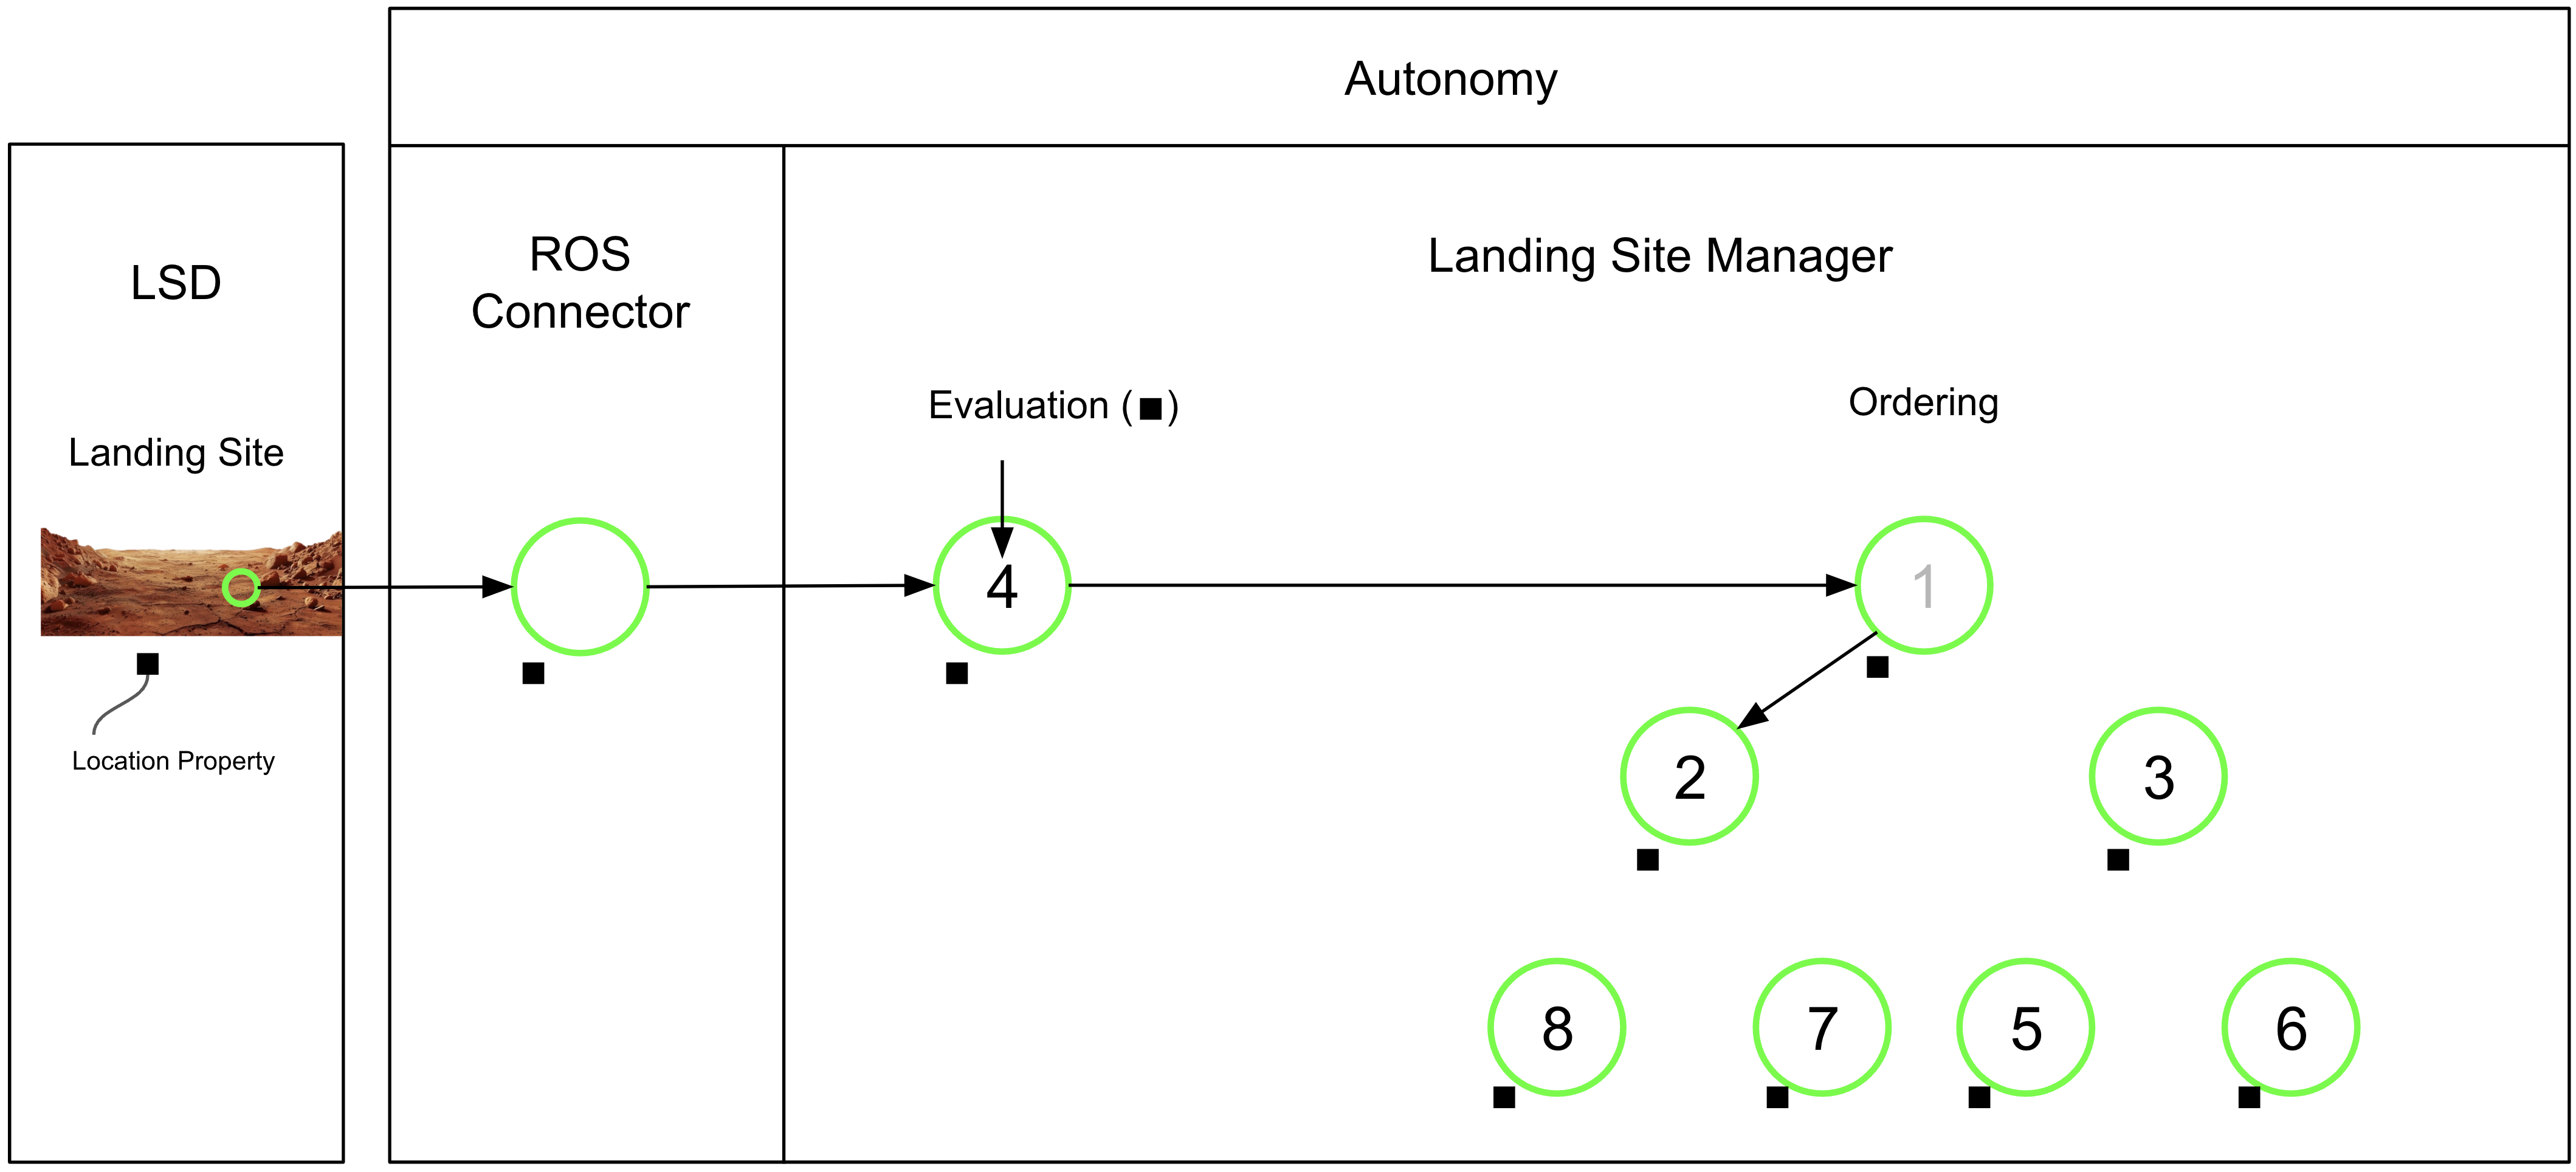
\includegraphics[scale=0.165]{images/system_overview/lsm_handling.png}
\caption{Landing site handling from detection to sorted position in the landing site manager: A landing site indicated with a green circle is detected by LSD and given to the autonomy with the location property. The landing site manager assigns the site a heuristic value based on the location and sorts it in the buffer array.}
\label{fig:lsm_ls_processing}
\end{figure}

Upon reaching the landing state and executing the landing behavior, the landing site buffer is ordered in descending order and the best landing site is returned which can then be used as the next navigation target to finally land at.

Both the landing site manager and the connector are implemented as singleton nodes for facilitated use throughout the entire autonomy framework. This means that they are accessible in every action performed by any state of the state machine without the need of instantiation of a landing site manager object instance. This is achieved by removing the copy constructor of the class as well as the assignment operator and creating an instance acquisition function, which returns a pointer to the single static instantiation of the class.

In this thesis the landing site manager was expanded significantly, both regarding the heuristics considered and the general handling of detected landing sites.

\subsubsection{Blackboard}\label{subsubsec:blackboard}

The blackboard is yet another singleton entity within the autonomy which allows the buffering of information to be shared between individual modules of the state machine.

It is implemented using a template based approach so that any variable can be directly stored and retrieved in a dynamic way without having to change the structure of the blackboard.

\subsection{Finite-State Machine}

Before going into the state machine implementation of the autonomy framework, the finite-state machine's working principle is explained:

\subsubsection{Working Principle}

A finite-state machine is a mathematical model of computation which allows the reactive implementation of a system with a finite number of states. It is defined by a finite set of possible states with an initial state, the transition rules in between these states, the events that trigger these transitions and the actions which are performed when the system is in a given state. It provides a very clearly structured implementation of the various states that a system can be in and is therefore a matching choice for the implementation of a rotorcraft mission.

A state machine continuously executes a tick. An executed tick carries out the action associated with the state that the state machine currently resides in. Depending on the output of that action, a transition event is triggered, moving the state machine from one state to another. This way the decision flow is propagated throughout the state machine until the behavior is concluded. This conclusive state in turn also has a transition which allows the state machine to start over again.

\subsubsection{The Finite-State Machine in the Autonomy Framework}

\begin{figure}[ht!]
    \centering
    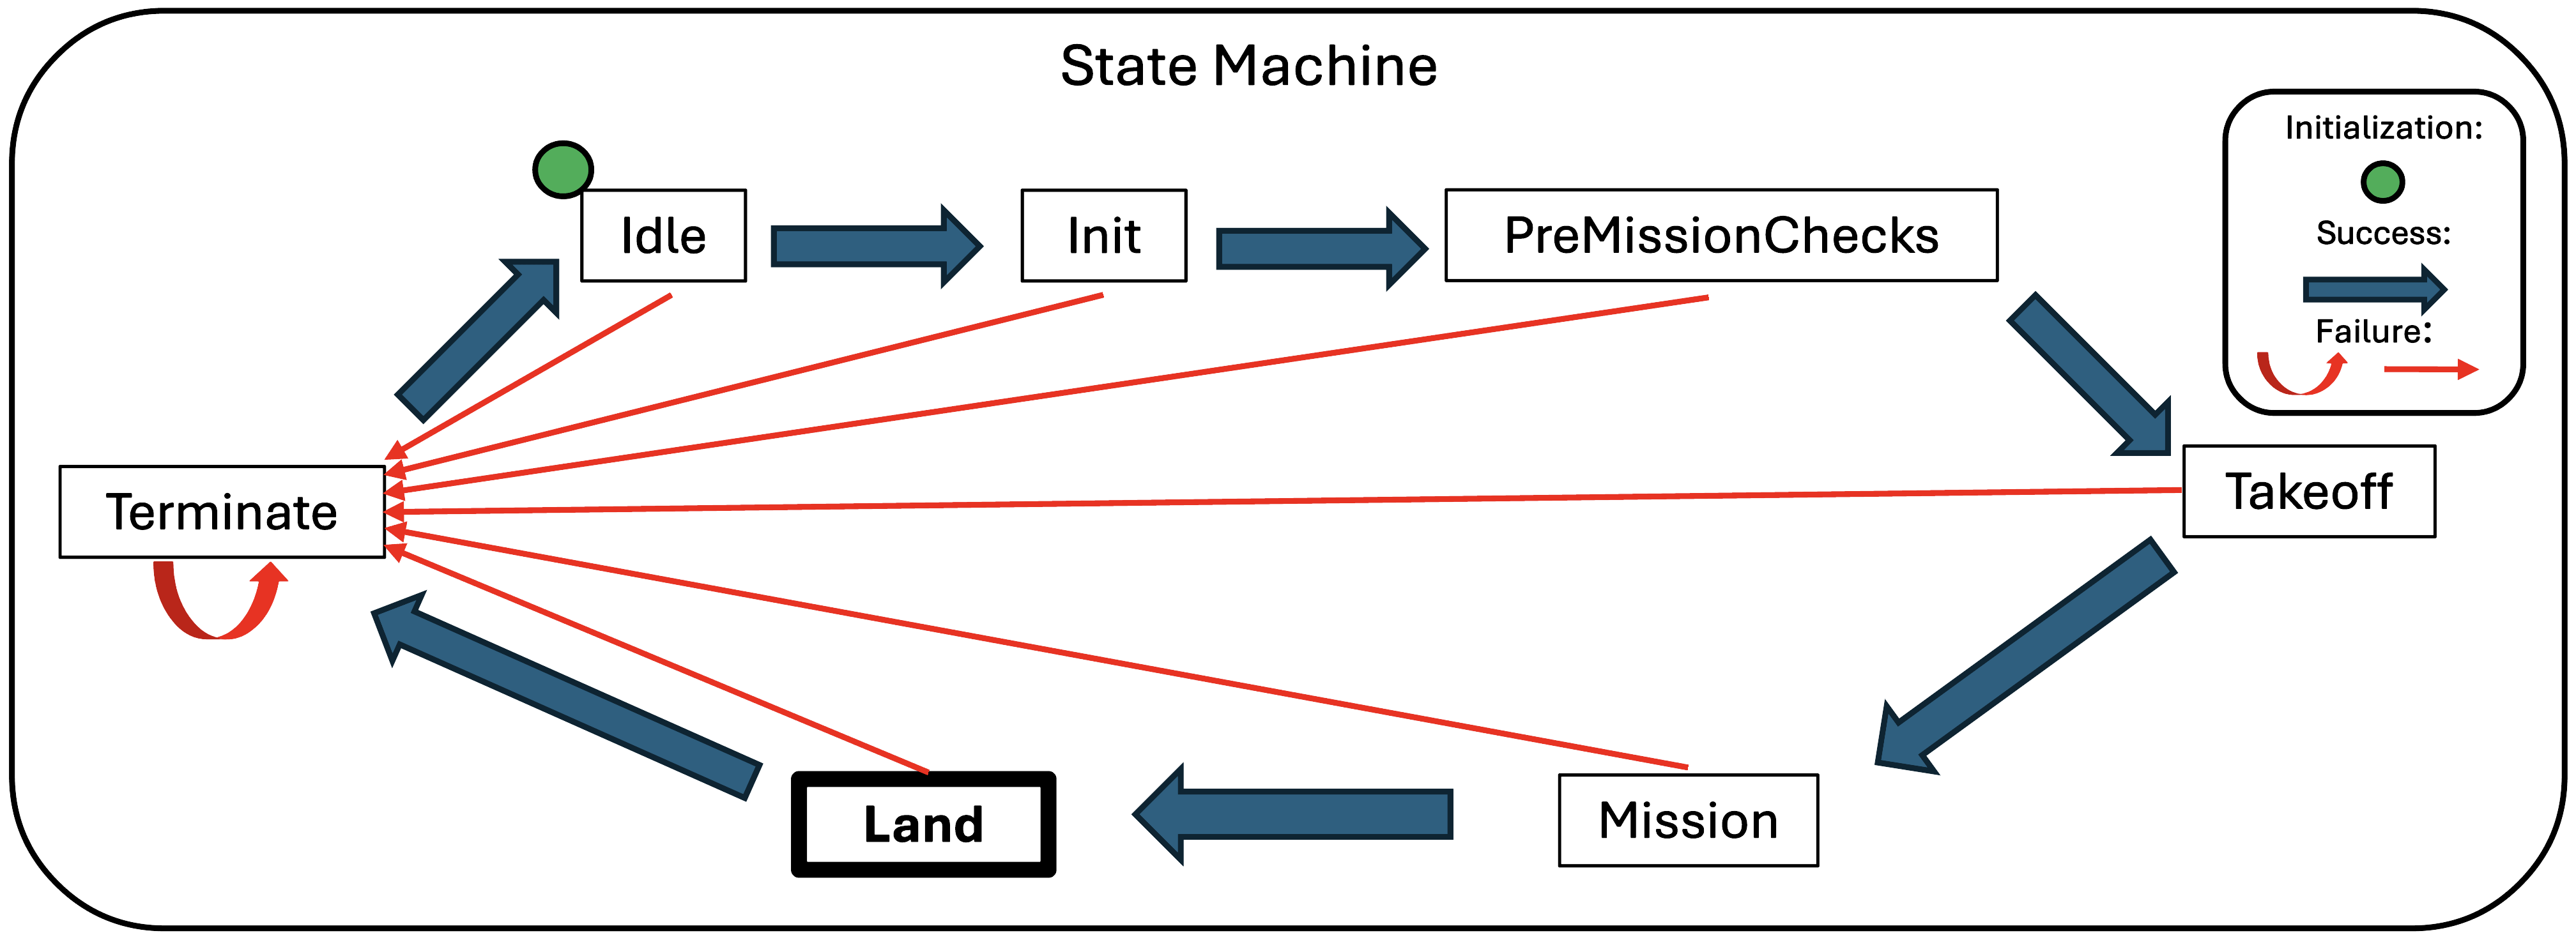
\includegraphics[scale=0.17]{images/system_overview/state_machine.png}
    \caption{State machine of the autonomy framework}
    \label{fig:state_machine}
\end{figure}

The autonomy continuously executes a tick. During nominal conditions, this simply denotes a tick in the finite-state machine. In the unfortunate case of a health event however, the state machine handles the health event based on in what state the FMS currently is. For instance, if it arises during initiation, the state machine simply transitions to the termination state, aborting the flight. In contrast, if the FSM's current state is the mission state, the rotorcraft immediately returns to the home position to land.

In each state during a state machine tick the respective behavior node is executed. Most often this is a single action node. For more complicated procedures a behavior tree is used. This is for instance the case for the landing state. For this thesis the landing node indicated in bold in \cref{fig:autonomy} is the most crucial part of the state machine. This is where the adaptive landing decisions are made to choose an adequate landing zone and orchestrate safe traversal to that location before finally landing on the surface.

\subsection{Behavior Tree}\label{subsec:setup:behavior_tree}

A behavior tree is a tool for systematic hierarchical plan execution. It enables the creation of complex tasks which are comprised of various simple tasks without having to worry about the implementation of such a small modular task. In that sense, it is similar to a finite-state machine.

However, in contrast to a state machine, nodes in a behavior tree are always executed in a hierarchical order. A node in a behavior tree is in one of three states at all times: 

\begin{itemize}
    \item RUNNING
    \item SUCCESS
    \item FAILURE
\end{itemize}

Being restricted to three states doesn't implicitly speak for the reactivity of the system. The more transition possibilities an entity has, the more reactive the system containing the entity is. However, the hierarchical execution flow of the nodes makes behavior tree's more easily scalable than finite-state machines. This is because the implementation of many transitions in a state machine quickly increases the complexity of the system. Action nodes in a behavior tree on the other hand can be organized in higher level control flow nodes which allows scalability of the system without a quick increase of complexity.

This is a matching choice of framework for the creation of complex modular flight behaviors. Especially since a rotorcraft mission can be easily split into small modular maneuvers such as ascension, lateral motion and rotation. Additionally, behavior trees allow anyone to draw up complex missions without the necessity of understanding the individual action node implementations in depth.

\subsubsection{Working Principle}
As the name suggests, a behavior tree can be visualized as a directed tree where the starting point of the tree is the root node. 

After the root node, three categories of tree nodes can follow:

\begin{itemize}
    \item Control flow nodes
    \item Action nodes
    \item Decorator nodes
    \end{itemize}
    
    Control flow nodes are comparatively higher level nodes which manage the execution flow of the behavior tree.
    
    The action nodes define the actual low level tasks performed in the broader behavior tree setup. 
    
    Lastly, the decorator nodes are auxiliary nodes which directly alter the workflow of action nodes in order to achieve smoother and more complex tree structures.
    
    Preceding nodes in a tree are called parent nodes while subsequently executed nodes are called child nodes of a node. A root node has no parent node and exactly one child node while control nodes have one parent node and potentially several child nodes. Action nodes are leaf nodes which have a parent node but no child nodes and decorator nodes have both one parent and one child node which they affect.

    Similarly to a state machine, the workflow of a behavior tree starts with the root node which continuously sends a tick signal to its child node. 

    

\subsubsection{Autonomy Control Flow Nodes}

The following control flow nodes are implemented:

\begin{itemize}
    \item Fallback Node
    
    Attempts to execute the first child node and if successful, it returns a success state. Else it continues to the next child node. If no child node was successful it returns the failure state. A boolean operator analogy for this would be the logical OR, stopping at the first successful entity.
    \item Sequence Node
    
    Executes one child after another. It only returns the SUCCESS state if all child nodes ran successfully. Otherwise, it returns false. Here an analogy would be the logical AND boolean operator.

    \item Parallel Node
    
    In this control flow node the child nodes are ticked in the hierarchical fashion as usual. However instead of waiting for the SUCCESS or FAILURE result of a given child node, its successor is already ticked. The parallel node returns SUCCESS if a predefined number of child nodes return SUCCESS or FAILURE in case a predefined number or all child nodes return FAILURE.
\end{itemize}

\subsubsection{Autonomy Decorator Nodes}\label{subsubsec:decorator_nodes}

The most important decorator nodes are:

\begin{itemize}
    \item Inverter Node
    
    Inverts the output of an action node. A boolean analogy would be the "!" (not) operator.
    \item Repeat Node
    
    Repeats a node a number of times until fails or a timeout is reached. 
    \item Retry Node
    
    Similar to the repeat node loop, but it repeats the node a number of times only until it succeeds, or a defined timeout is reached.
    \item Timeout Node
    
    Adding a timeout to an action node which otherwise wouldn't be temporally limited.
\end{itemize}

\subsubsection{Autonomy Action Nodes}\label{subsubsec:setup:action_nodes}

There are a multitude of actions required for the various subtask a rotorcraft has to perform during a mission. The most important ones for the landing behavior in this work are the following:

\begin{itemize}
    \item ChangeAltitudeAction
    
    Changes the drone's altitude to the given value. The ascend / descend velocity diminishes upon reaching proximity to the desired waypoint.
    \item HoldPoseAction
    
    Self-explanatory: the drone holds the current pose for a given time.
    \item LandingAction
    
    Similar to the ChangeAltitudeAction, it descends to a waypoint which in this case is simply the ground vertically below the drone's current position. Upon reaching a certain proximity to the landing point, the descent velocity is reduced to a minimum in order to accomplish smooth landing.
    \item NavigateToWaypointAction
    
    Lateral movement to the given waypoint. Same proximity based slow-down mechanism as ChangeAltitudeAction and LandingAction.
    \item RotateTowardsWaypointAction
    
    Rotates the drone to face the given waypoint.
\end{itemize}

\subsubsection{Behavior Tree Example}\label{subsubsec:BT_exp}

An example of a simple behavior tree is shown in \cref{fig:BT_exp}.

\begin{figure}[h]
\centering
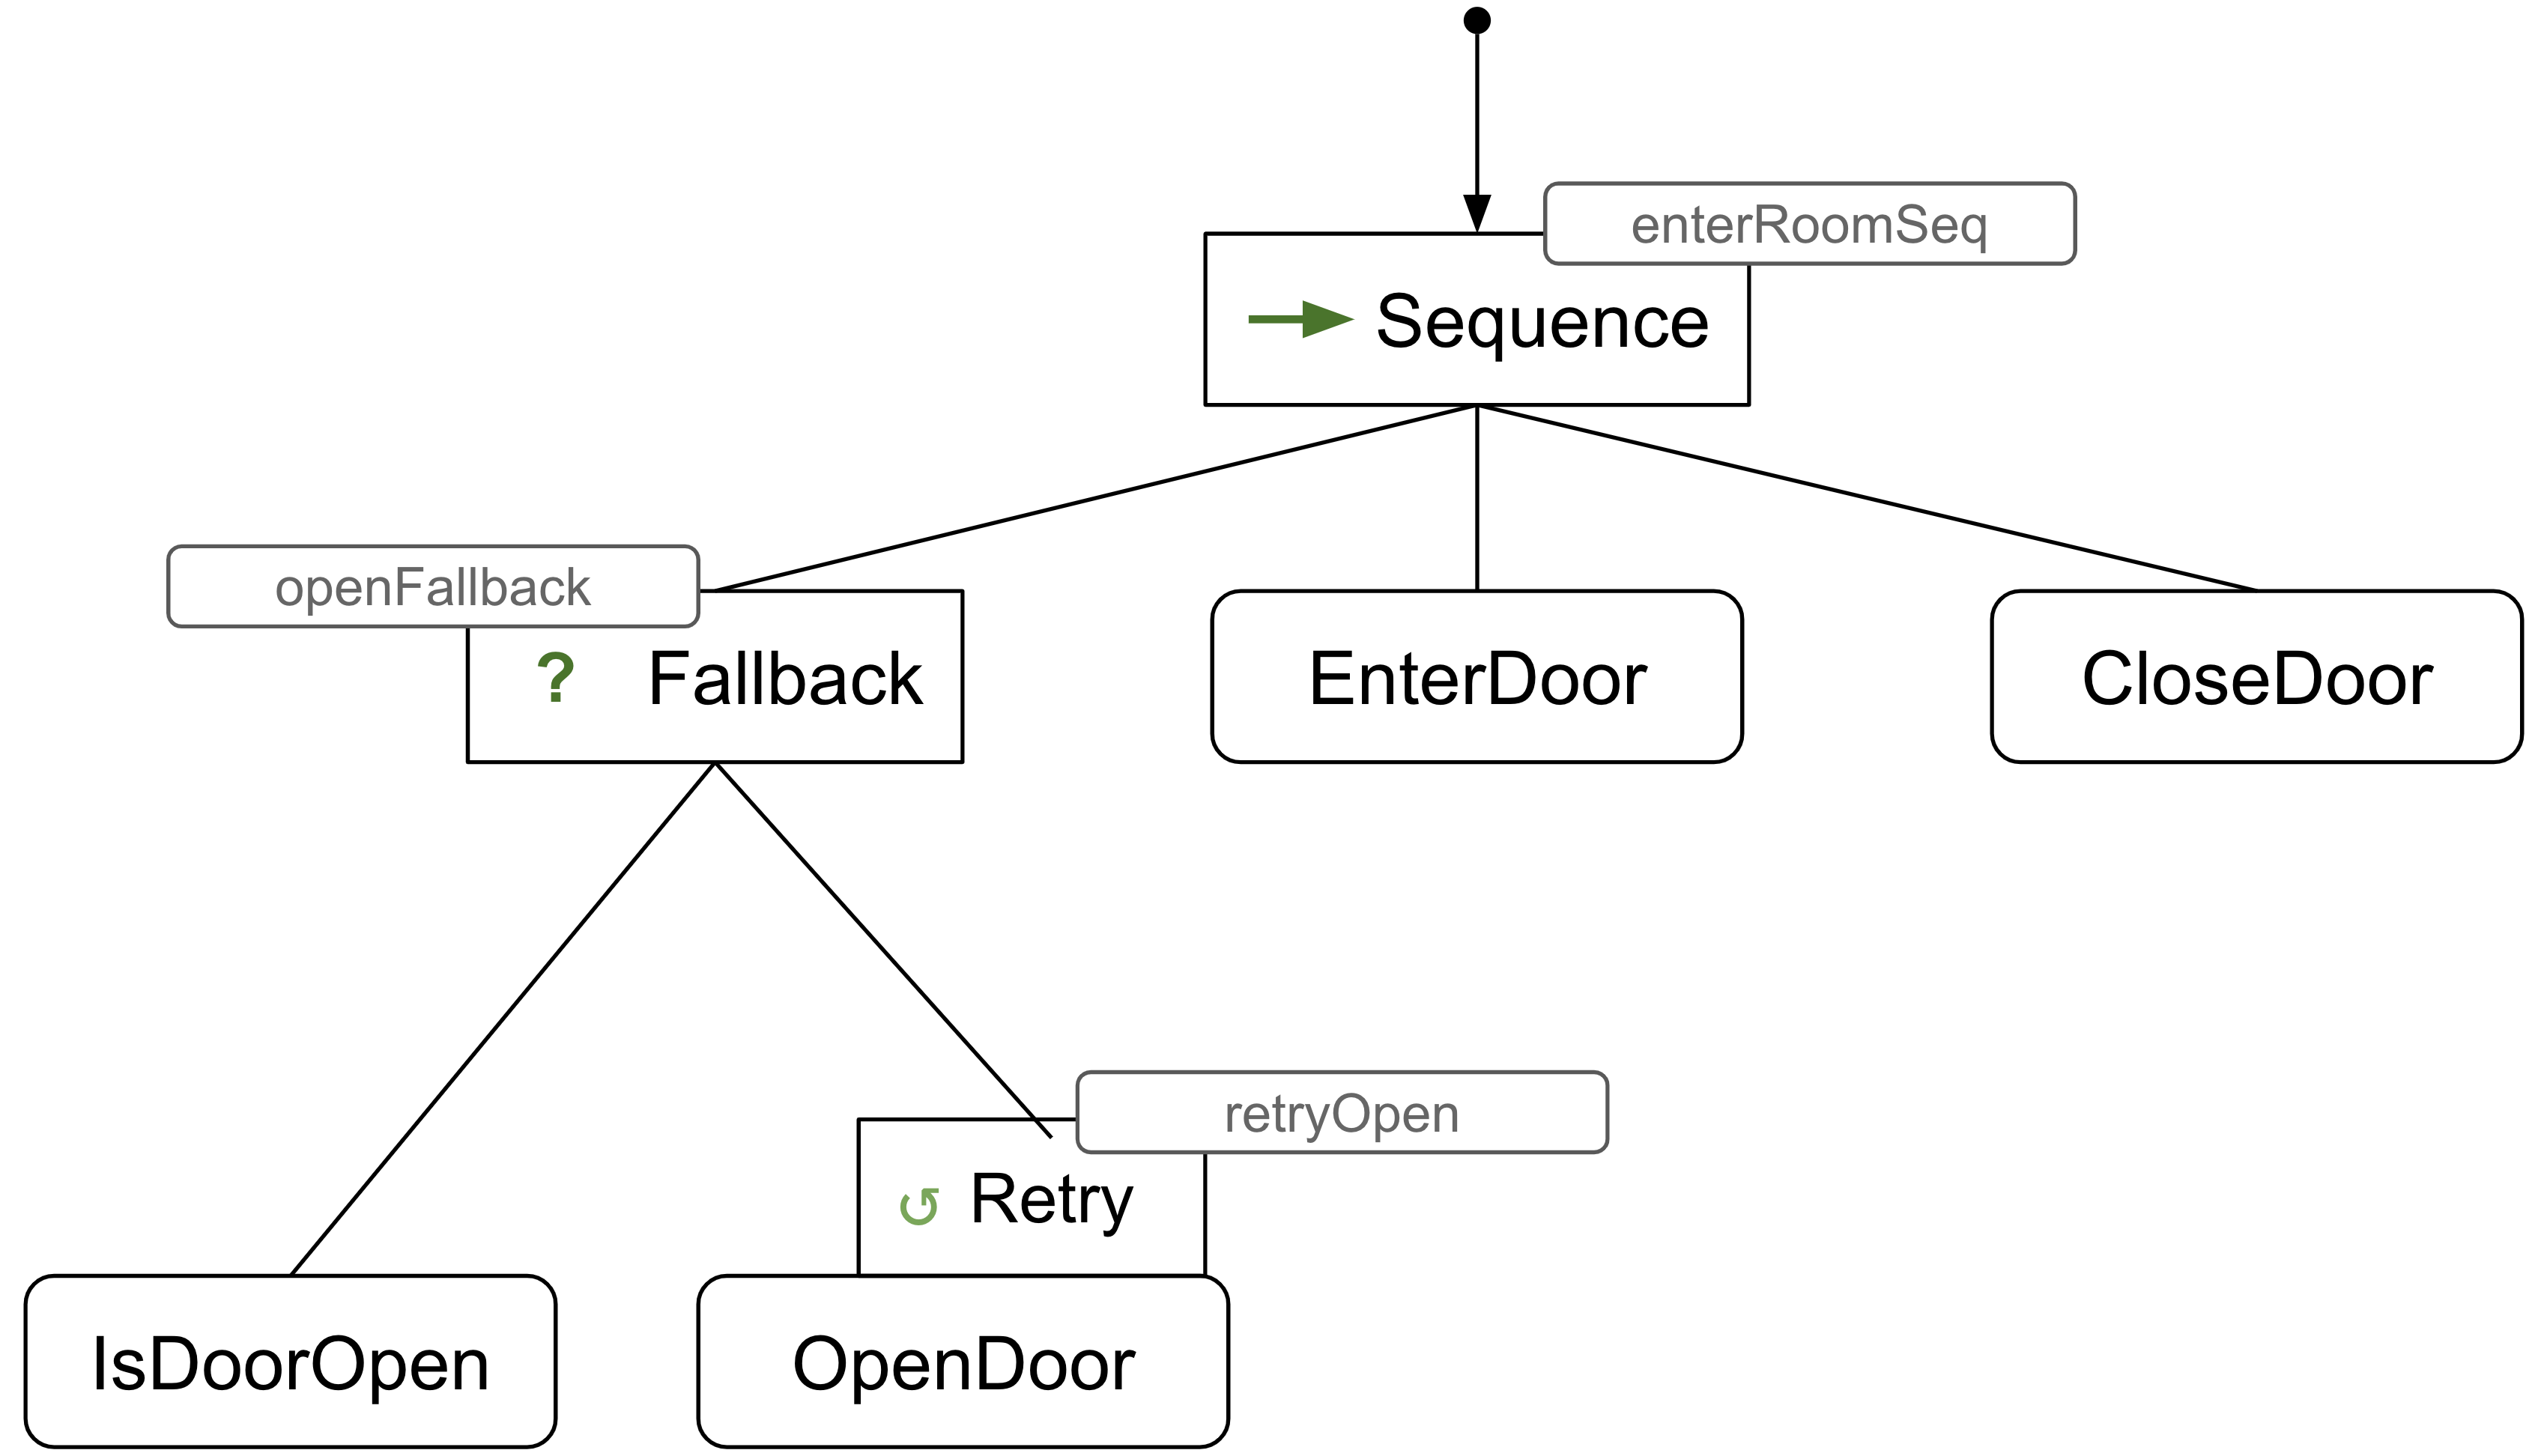
\includegraphics[scale=0.2]{images/system_overview/BT_example.png}
\caption{Simple, often used behavior tree example of entering a room}
\label{fig:BT_exp}
\end{figure}

Big, rectangular boxes indicate control flow nodes while boxes with round edges are action nodes and small rectangles attached to action nodes are decorator nodes. To distinguish the control flow nodes from each other, their name is attached.

In this example, the root node, depicted as a black circle, initiates a sequence node. The sequence node executes all of its child nodes one by one. The first is a fallback node which checks whether the door is already open using the IsDoorOpen action. If it returns successfully, the fallback node concludes the state success and the rest of the sequence node can be executed. If not, the tree repeatedly attempts to open the door using the Retry decorator node. Either the door opens or the fallback node and therefore also the sequence node fail. Lastly, if the door eventually opens, the other actions of entering and closing the door can be performed.






